%\documentclass[twocolumn]{fairmeta}
% Option "twocolumn" available, but please prioritize single-column
\documentclass[onecolumn]{fairmeta}
\usepackage[most]{tcolorbox}

\usepackage{amsmath}
\usepackage{amssymb}


\newcommand{\QG}[1]{\textcolor{red}{QG:~#1}}
\newcommand{\TN}[1]{\textcolor{orange}{TN:~#1}}
\newcommand{\NB}[1]{\textcolor{blue}{NB:~#1}}
\newcommand{\MR}[1]{\textcolor{magenta}{MR:~#1}}

\title{\algoname{}: Towards Functional Tool-Use Generalization via Keypoint Trajectory Reasoning}

% ORDER TBD
\author[1]{Chuhao Zhou}
\author[2]{Liquan Wang}
\author[2]{Shuxin Cao}
\author[1]{Xiangyu Chen}
\author[1]{Yuxuan Hu}
\author[1]{Boyu Ma}
\author[2]{Animesh Garg}
\author[1, \dagger]{Jianfei Yang}


\affiliation[1]{MARS Lab, Nanyang Technological University}
\affiliation[2]{Georgia Institute of Technology}


%\contribution[*]{Work done at Meta}
\contribution[\dagger]{Corresponding Author}

\usepackage{graphicx}
\usepackage{amsmath}
\usepackage{amsfonts}
\usepackage{booktabs}
\usepackage{multirow} 
\usepackage[table]{xcolor}
\usepackage{wrapfig}
\usepackage{caption}
\usepackage{placeins}
% \usepackage{xspace}

%%%%%%%%%%%%%%%%%%%%%%%%%%%%%%%%
% ADD COMMAND
%%%%%%%%%%%%%%%%%%%%%%%%%%%%%%%%
\usepackage{xcolor}
\usepackage{enumitem}
\definecolor{cPink}{RGB}{255,105,180}
\newcommand{\lw}[1]{\textcolor{cPink}{[LW: #1]}}
\newcommand{\algoname}{\textsc{FuncBridge}}


\abstract{
While humans readily repurpose a book, a stone, or a shoe to drive a nail, robots trained on specific tools fail to transfer the same function to novel ones -- a gap we formalize as \textit{functional generalization}.
Functionally equivalent tools share visually recognizable functional intent, such as where contact can occur and how a contact region should move to the target. However, this perceptual similarity does not directly carry over to action space, where each tool demands a different motor pattern to realize the function.
To bridge this gap, we explore intermediate representations including affordance images, human video prompts, functional videos and object masks, and 2D keypoint trajectories, finding that keypoint trajectories best balance functional expressiveness and action groundability. 
Building on this, {we present \algoname{}, a two-stage framework} that decouples functional reasoning from action execution: learning to predict generalizable keypoint trajectories from action-free data, then grounding them into robot actions with limited demonstrations. 
Across a benchmark spanning ten tools and three functions, including hitting, sweeping, and hooking, \algoname{} consistently outperforms state-of-the-art methods on unseen tools in both simulation and the real world.
}

% \hypersetup{
%     colorlinks=true,
%     linkcolor=red,
%     citecolor=cyan,
%     filecolor=magenta,      
%     urlcolor=magenta,
% }
    
\correspondence{Jianfei Yang at \email{jianfei.yang@ntu.edu.sg}}
% You can add additional metadata fields as follows
\metadata[Project Page]{\url{https://chuhaozhou99.github.io/FuncBridge/}}

%===============================================================================
\begin{document}
\maketitle

%===============================================================================

%===============================================================================
\section{Introduction}
\label{sec:intro}
	 
In open-ended real-world environments, the right tool is rarely at hand, yet humans adapt effortlessly by repurposing available objects to accomplish functions. For example, in hitting, a book, a stone, or a shoe can be used to drive a nail because functionally equivalent tools share a common functional intent: a contact region to strike with and a motion that brings it onto the target. 
This capacity, which we term \textit{functional generalization}, is a hallmark of human dexterity that robots have yet to achieve. Current manipulation policies overfit to the appearance and geometry of seen tools, failing when handed a novel one that serves the same function~\citep{chen2025tool, turpin2021gift, qin2023robot, jia2026action, bai2026flash}.

\begin{figure}[ht]
    \centering
    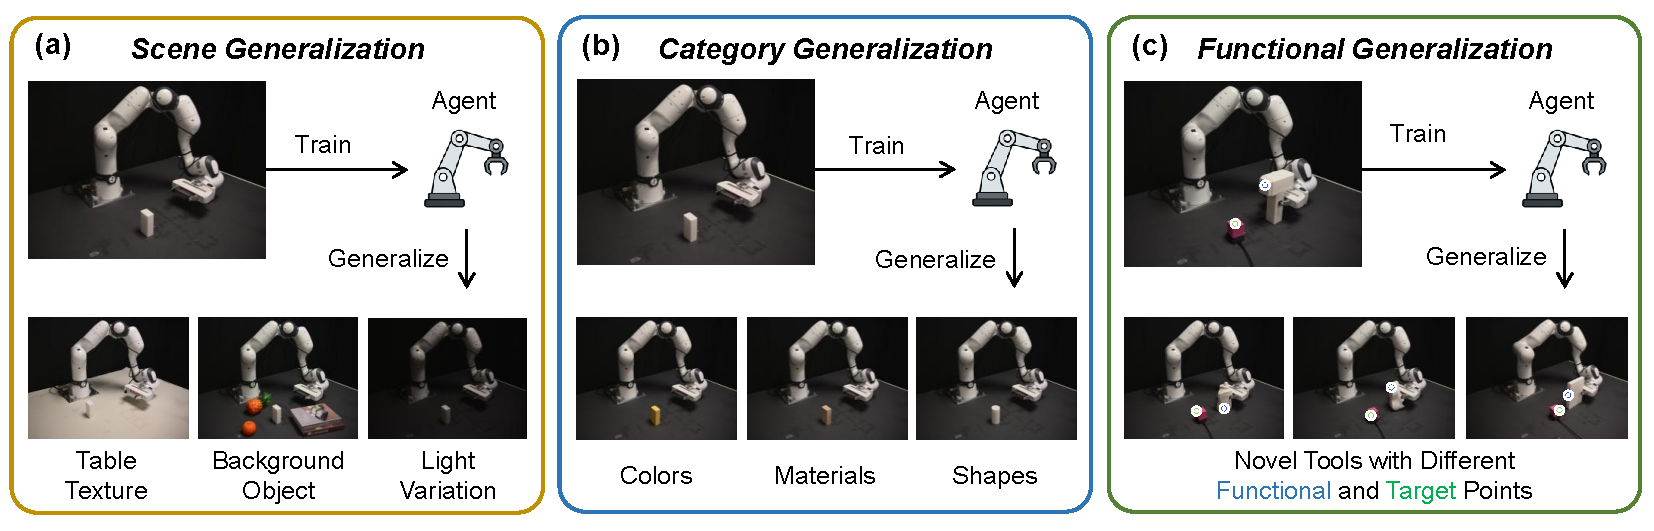
\includegraphics[width=1.0\linewidth]{figures/teaser_v2.pdf}
    % \caption{
    % \textbf{Comparison between functional generalization and existing generalization settings.}
    % (a) Scene generalization evaluates robustness to visual variations.
    % (b) Category generalization tests transfer across objects with diverse properties.
    % (c) Functional generalization requires using unseen tools to accomplish the same function.
    % }
    \caption{
    \textbf{Comparison of functional generalization with existing generalization settings.}
    (a) Scene generalization handles visual variations.
    (b) Category generalization transfers across object properties.
    (c) Functional generalization uses unseen tools for the same function.
    }
    \label{fig:functional_generalization}
\end{figure}
Functional generalization is fundamentally harder than conventional generalization. As illustrated in Fig.~\ref{fig:functional_generalization}, scene- and category-level generalization require tolerating visual variations while the underlying motion stays the same~\citep{goyal2023rvt, shridhar2023perceiver, shridhar2022cliport, nair2023r3m}. Functional generalization, by contrast, {demands adapting the motion to each tool's geometry}: striking a target with a novel tool requires locating its contact region, aligning it, and producing an appropriate motion, even when the tool's shape and required trajectory differ from training. {The core difficulty is a mismatch: functionally equivalent tools exhibit common functional intent that can be perceived from visual observations, but realizing the same function requires different motions across tools.}


%Bridging this perception-to-action gap requires an intermediate representation that carries functional intent across tools, satisfying two competing demands:  expressive enough to capture where to make contact and how to move onto the target, yet grounded enough to be predicted from \textcolor{cBlue}{perceived} observations without overfitting to tool-specific appearance. 
Bridging this perception-to-action gap requires an intermediate representation that carries functional intent across tools, satisfying two competing demands: {it should be expressive enough to capture where contact can occur and how a selected contact region should move toward the target, yet abstract enough to discard tool-specific appearance that may hinder generalization to unseen tools.}
Dense representations like raw video entangle function-relevant cues with tool-specific appearance, while overly sparse ones discard the geometric and temporal structure needed for precise action grounding. This trade-off raises the central question of our work: \textit{which representation best transfers functional intent from perception to action?}

To answer this question, we evaluate intermediate representations 
including affordance images, human video prompts, {functional videos and object masks}, and 2D keypoint trajectories, 
finding that keypoint trajectories best balance functional expressiveness and 
action groundability: they capture function-relevant contact and motion structure 
while discarding tool-specific appearance that causes overfitting. Building on 
this, we propose \algoname{}, a two-stage framework that 
decouples functional reasoning from action execution.
%it first predicts  generalizable keypoint trajectories for unseen tools from large-scale action-free data, then grounds these functional plans into executable robot actions using a small set of action-labeled demonstrations. 
{It learns a functional keypoint predictor from large-scale action-free data and an action-grounding policy from limited action-labeled demonstrations. At inference, the predictor predicts function-relevant keypoint trajectories, which the execution policy grounds into robot actions.
We further introduce a benchmark spanning ten tools and three functions, including hitting, sweeping, and hooking, on which \algoname{} consistently outperforms state-of-the-art methods on unseen tools in both simulation and the real world, achieving substantial gains in average success rate.}
In summary, our contributions are threefold:
\begin{itemize}[leftmargin=*]
    \item We formalize \textit{functional generalization} in robotic tool-use and identify the perception-to-action gap as its core difficulty.
    \item We find that 2D keypoint trajectories best balance functional 
    expressiveness and action groundability, and propose \algoname{}, {a two-stage framework that learns functional keypoint planning from action-free data and action grounding from limited robot demonstrations.}
    % \textcolor{cBlue}{\item Through extensive simulation experiments across 10 tools and three functions, together with real-world validation, we demonstrate that \algoname{} consistently outperforms state-of-the-art methods on unseen tools.}
   {\item Across ten tools and three functions in simulation, with real-world validation, we demonstrate that \algoname{} consistently outperforms state-of-the-art methods on unseen tools.}
\end{itemize}




%===============================================================================

\section{Related Works}
\label{sec:related_works}

\paragraph{Generalization Problems in Robotic Manipulation.}
Generalization has been a central problem in robotic manipulation, and existing studies mainly evaluate it from three perspectives: scene-level, category-level, and cross-embodiment generalization.
Scene-level generalization focuses on whether a policy can remain robust when the surrounding visual or physical contexts vary, such as changes in object layouts, lighting conditions, or camera viewpoints~\citep{goyal2023rvt, shridhar2023perceiver, shridhar2022cliport, nair2023r3m}. 
Category-level generalization studies whether robots can transfer manipulation skills to unseen objects that belong to the same semantic category while differing in geometry, size, or texture~\citep{gao2021kpam, mo2021where2act, geng2023gapartnet}.
More recently, cross-embodiment generalization has attracted attention, which aims to train a unified policy that can transfer across different robot platforms, such as robotic arms and humanoids~\citep{o2024open, team2024octo, intelligence2025pi}.
In this work, we go beyond generalization over visual appearance and robot embodiment and focus on \textit{functional generalization}, in which an agent is required to accomplish the same function using diverse, unseen tools.


\paragraph{Improving Generalization in Robot Policy Learning.}
To improve manipulation generalization, the most straightforward way is scaling up action-labeled robotic data and training policies end-to-end~\citep{zitkovich2023rt, o2024open, team2024octo, khazatsky2024droid, jia2026physics}. 
However, collecting large-scale robotic data is time-consuming and labor-intensive, especially for complicated tool-use manipulations. 
Reducing the dependence on action labels, some works learn transferable motion priors from large-scale action-free video data~\citep{nair2023r3m, wang2023mimicplay, wu2024unleashing,ma2026dit4dit, pai2025mimic, an2026feedback, hou2026world}. 
For example, MimicPlay~\citep{wang2023mimicplay} learns high-level latent plans from human play videos and grounds them into robot actions with a low-level visuomotor policy. 
Although videos contain rich motion and interaction cues, dense future frames do not explicitly reveal a compact abstraction of function-relevant intent. As a result, effectively learning functional priors from videos often requires extremely extensive pretraining.
Another line of work improves action grounding with more structured intermediate representations, such as interaction heatmaps~\citep{mo2021where2act, bahl2023affordances, wu2025afforddp, li2026compassad}, task-oriented grasps~\citep{fang2020tog}, object-centric representations~\citep{zhulearning, chen2025tool, chapin2025object, cao2026keygen}, or keypoint trajectories~\citep{gao2021kpam, huang2025rekep, turpin2021gift, wen2023any, cao2026keygen}.
For instance, ATM~\citep{wen2023any} predicts future trajectories of arbitrary points from video and uses them to guide a low-level policy for action generation. 
However, these methods mainly focus on standard manipulation tasks, such as object pick-up, while overlooking tool-use scenarios that require capturing more abstract functional intent, which are systematically investigated in our work. 





% through the lens of different intermediate representations.
% However, these methods mainly focus on standard manipulation tasks, such as object pick up, while overlooking tool-use scenarios that require understanding more abstract functional intent. 
% In this work, we systematically investigate the effect of different intermediate representations on functional generalization and identify that keypoint trajectories provide the best trade-off between visual predictability and action groundability.

%\paragraph{Intermediate Representations for Tool-use Manipulation.}
% Instead of directly predicting low-level actions from raw observations, many manipulation methods introduce intermediate representations to provide more structured guidance. Affordance-based methods identify task-relevant object regions for interaction, while keypoint-based methods represent objects or tools using sparse semantic points to support category-level manipulation and action grounding. Other works use human videos or predicted future observations as high-level plans, which can capture task intent before execution. These intermediate signals improve interpretability and transferability, but they often differ in visual predictability and action groundability. For contact-rich tool-use tasks, an effective representation should not only capture where the functional interaction occurs, but also describe how the tool should move over time. In this work, we systematically study several candidate representations, including affordance images, human video prompts, and 2D keypoint trajectories, and show that keypoint trajectories provide a better trade-off between functional planning and executable action grounding.

% Improving the generalization capability of robotic policies is a central challenge for deploying robots in open-world environments. Existing methods mainly address this problem from three perspectives.

% \paragraph{Scaling up Robotic Data.}
% One direct way to improve generalizable planning is to scale up robotic demonstrations and train policy models end-to-end to predict actions from observations~\cite{}. For example, Open X-Embodiment~\cite{} aggregates large-scale robot trajectories from many laboratories and enables RT-X to learn transferable skills across tasks and embodiments. Similarly, Octo~\cite{} trains a generalist policy on heterogeneous robot datasets and shows strong multi-task manipulation ability. However, collecting large-scale robot data is extremely labor-intensive and time-consuming, and the resulting policies may still lack explicit functional abstraction beyond the demonstrated objects and scenes.

% \paragraph{Pretraining on Human Videos.}
% Another direction is to pretrain policy models on action-free human videos to learn motion priors, and then transfer these priors to robot action generation through fine-tuning on a small amount of robotic demonstrations. For instance, R3M~\cite{} learns reusable visual representations from large-scale human videos and transfers them to downstream robot manipulation tasks. MimicPlay~\cite{} further extracts high-level plans from human play videos and grounds them with a low-level robot policy. However, without explicit action or physical supervision, it is difficult for models to learn the precise dynamics required for motor control, which may require extremely large-scale video pretraining.

% \paragraph{Exploiting Foundation Models.}
% Another stream of works~\cite{} uses pretrained foundation models to extract generalizable affordance or planning signals, which serve as intermediate bridges between seen and unseen demonstrations. For example, RT-H~\cite{} leverages vision-language reasoning to predict action hierarchies, allowing high-level semantic plans to guide low-level robot execution. Large Video Planner further takes a video foundation model as a high-level planner to predict future visual plans, which are then grounded into robot actions by a low-level policy. However, using foundation models during inference can introduce significant latency, and the final policy performance is strongly limited by the accuracy of the predicted intermediate signals.

% \paragraph{Summary.}
% Beyond data-centric strategies, recent methods~\cite{} exploit pretrained foundation models to extract generalizable affordance or planning signals, which serve as intermediate bridges between seen and unseen demonstrations. The goal is to enable a policy to transfer the same functional behavior, such as hitting, to novel tools with different shapes, materials, and interaction regions. To this end, we propose an efficient System-2 plus System-1 architecture, where System-2 predicts generalizable intermediate functional plans and System-1 grounds these plans into executable robot actions. This design aims to bridge high-level functional reasoning and low-level action execution, thereby improving policy generalization beyond object-specific imitation.


%===============================================================================

\begin{figure}[ht]
    \centering
    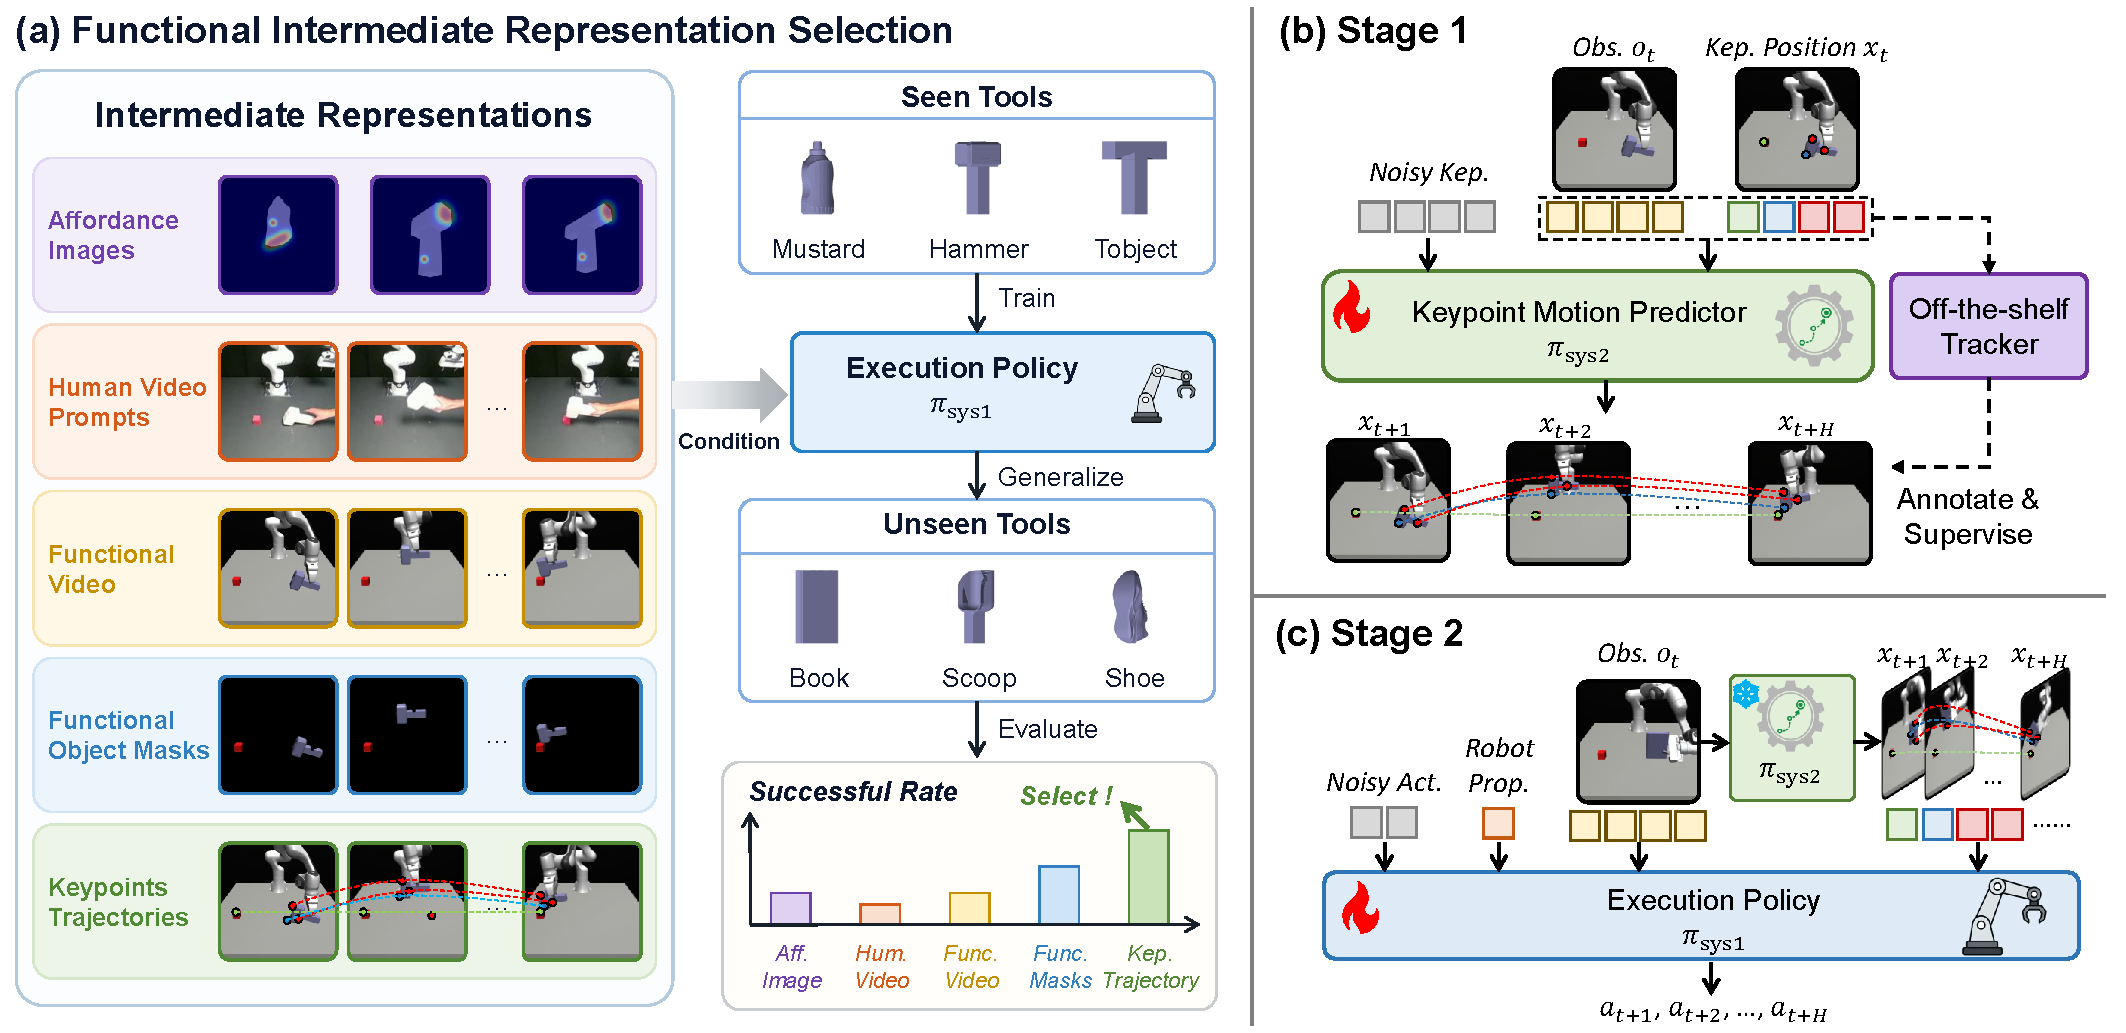
\includegraphics[width=0.95\linewidth]{figures/main_pipeline_v2.pdf}
    \caption{
    \textbf{Overview of the \algoname{}.} (a) Evaluation and selection of functional intermediate representations. (b) In Stage 1, the System-2 planner learns to predict future keypoint-based functional plans from action-free observations. (c) In Stage 2, the System-1 execution policy grounds the predicted functional plans into executable robot actions.
    }
    \label{fig:functional_generalization_pipeline}
\end{figure}

\vspace{-15pt}
\section{Methods}
\label{sec:method}



\subsection{Problem Formulation}
We formulate functional generalization in tool-use manipulation as a Markov Decision Process (MDP), where the state $\mathbf{s}_t$ consists of the visual observation $\mathbf{o}_t$, the proprioceptive state $\mathbf{q}_t$, and optionally a functional intermediate representation $\mathbf{x}_t$ (e.g., keypoint trajectories) that carries function-relevant cues bridging perception and action, and the action $\mathbf{a}_t$ is the motor command. A task function (e.g., hitting a target) is defined over seen tools $\mathcal{T}_{\text{seen}}$ for training and disjoint unseen tools $\mathcal{T}_{\text{unseen}}$ for evaluation, where the function stays fixed but the tool, its appearance, and the required contact positions and motions all change.


Two types of data are available for learning. The first is an action-free dataset $\mathcal{D}_{U}=\{(\mathbf{O}^{(i)}, \mathbf{X}^{(i)})\}_{i=1}^{N_U}$, consisting of visual observations $\mathbf{O}^{(i)}=\{\mathbf{o}^{(i)}_t\}_{t=1}^{T}$ and functional intermediate representations $\mathbf{X}^{(i)}=\{\mathbf{x}^{(i)}_t\}_{t=1}^{T}$, which is abundant and can span a broader range of tools since it requires no robot labels.
The second is a smaller action-labeled robotic dataset $\mathcal{D}_{L}=\{(\mathbf{O}^{(i)}, \mathbf{X}^{(i)}, \mathbf{Q}^{(i)}, \mathbf{A}^{(i)})\}_{i=1}^{N_L}$, which provides proprioceptive states $\mathbf{Q}^{(i)}$ and ground-truth actions $\mathbf{A}^{(i)}$ but is costly to collect, so $|\mathcal{D}_L| \ll |\mathcal{D}_U|$. This data asymmetry, together with the perception-to-action gap discussed in Sec.~\ref{sec:intro}, motivates a two-stage decomposition: 
\begin{equation}
\underbrace{
\pi_{\mathrm{FuncBridge}}(
\mathbf{a}_{t:t+H} \mid \mathbf{o}_{t}, \mathbf{q}_{t}, \mathbf{x}_{t}
)
}_{\text{FuncBridge}}=
\underbrace{
\pi_{\mathrm{sys2}}(
\hat{\mathbf{X}}_{t:t+H} \mid \mathbf{o}_{t}, \mathbf{x}_{t}
)
}_{\text{functional reasoning}}
\underbrace{
\pi_{\mathrm{sys1}}(
\mathbf{a}_{t:t+H} \mid \mathbf{o}_{t}, \mathbf{q}_{t}, \hat{\mathbf{X}}_{t:t+H}
)
}_{\text{grounded execution}} .
\label{eq:forge_decomposition}
\end{equation}
% \algoname{} learns a future-state predictor on $\mathcal{D}_U$ that forecasts the functional intermediate representation from observations, and an execution policy on $\mathcal{D}_L$ that grounds the predicted representation into robot actions.
\algoname{} learns a future predictor on $\mathcal{D}_U$ for forecasting functional intermediate representations from observations, and an execution policy on $\mathcal{D}_L$ for grounding representations into actions.

%(e.g., 2D keypoint trajectories from an off-the-shelf tracker),  





\subsection{Functional Intermediate Representations Selection}
\label{sec:Functional Intermediate Representations Selection}
As discussed in Sec.~\ref{sec:intro}, a desired functional intermediate representation $\mathbf{X}_{t:t+H}$ should preserve the contact and motion structure shared across tools, while remaining predictable from action-free observations and groundable into precise robot actions. 
We hypothesize that 2D keypoint trajectories form a suitable choice of $\mathbf{X}_{t:t+H}$. 
They discard tool-specific appearance that may cause overfitting, while retaining compact geometric information such as the contact point, target position, and affordance-relevant tool structure. 
At the same time, they provide a structured temporal description of how function-relevant points should move, which makes them easy to predict from existing vision models~\citep{wen2023any} and to ground into actions. 
% To validate this hypothesis, we compare keypoint trajectories with two alternative choices of $\mathbf{X}_{t:t+H}$: affordance images and human video prompts.
{To validate this hypothesis, we compare keypoint trajectories with four alternative choices of $\mathbf{X}_{t:t+H}$ spanning different temporal forms as shown in Fig.~\ref{fig:functional_generalization_pipeline}: affordance images as static conditions, human video prompts as pooled conditions, and functional videos and object masks as sequential conditions.}


\textbf{Affordance Image.}~~
Given an affordance image $I_{\mathrm{aff}}^{(i)}$, we encode it with an image encoder $E_{\mathrm{img}}$~\citep{he2016deep} and use the resulting feature as a time-invariant condition: $x_t^{(i)}=E_{\mathrm{img}}(I_{\mathrm{aff}}^{(i)})\in\mathbb{R}^{d}$.

\textbf{Human Video Prompt.}~~
Given a human video $V_{\mathrm{hum}}^{(i)}=\{I_{\mathrm{hum},t}^{(i)}\}_{t=1}^{T}$, we encode it with a video encoder $E_{\mathrm{vid}}$~\citep{bertasius2021space} and apply temporal average pooling to obtain a sequence-level feature, which is used as a time-invariant condition: $x_t^{(i)}=\mathrm{AvgPool}(E_{\mathrm{vid}}(V_{\mathrm{hum}}^{(i)}))\in\mathbb{R}^{d}$.

{\textbf{Functional Videos and Object Masks.}~~
Given a ground-truth functional execution video $V_{\mathrm{func}}^{(i)}=\{I_{\mathrm{func},t}^{(i)}\}_{t=1}^{T}$, we encode each frame with an image encoder $E_{\mathrm{img}}$, yielding a temporally varying condition $x_t^{(i)}=E_{\mathrm{img}}(I_{\mathrm{func},t}^{(i)})\in\mathbb{R}^{d}$. For object masks, as shown in Fig.~\ref{fig:functional_generalization_pipeline}, we remove the background while retaining the tool and target object in each frame, with the masked frames encoded similarly.}


\textbf{Keypoint Trajectory.}~~
We denote the keypoint trajectory as $P^{(i)}=\{p_t^{(i)}\}_{t=1}^{T}$, where each frame $p_t^{(i)}=\{p_t^{(i),k}\}_{k=1}^{K}$ contains $K$ 2D keypoints.
At time step $t$, we flatten the keypoint coordinates and encode them with a keypoint encoder $E_{\mathrm{kp}}$, yielding $x_t^{(i)}=E_{\mathrm{kp}}(\mathrm{Flatten}(p_t^{(i)}))\in\mathbb{R}^{d}$.


To evaluate these candidates, we conduct a provided-reference experiment in Fig.~\ref{fig:functional_generalization_pipeline}~(a), where each representation is pre-extracted for both seen and unseen tools and used as the condition for the execution policy $\pi_{\mathrm{sys1}}$. The policy is trained on action-labeled data from seen tools in $\mathcal{D}_{L}$ and evaluated on unseen tools for hitting, where a rollout is successful if the designated hitting region strikes the target. Among candidates, 2D keypoint trajectories achieve the best performance, since they go beyond static region cues and dense visual motion by providing a compact, structured description of how function-relevant points move and align over time. We therefore adopt 2D keypoint trajectories as the functional intermediate representation for \algoname{}.




%\subsection{Functional Reasoning and Grounded Execution Policy}
% \subsection{{\algoname{} Framework}}
\subsection{\algoname{}: Two-Stage Functional Reasoning and Grounded Execution}
\label{sec:FORGE}
After selecting 2D keypoint trajectories as the functional intermediate representation, we design a two-stage framework to decouple functional reasoning from action execution.
This enables \algoname{} to learn transferable functional keypoint motion from action-free demonstrations, while grounding the predicted trajectories into robot actions with limited action-labeled data.


\textbf{Stage 1: Action-free Functional Reasoning.}~~ 
As shown in Fig.~\ref{fig:functional_generalization_pipeline}~(b), we train the keypoint motion predictor $\pi_{\mathrm{sys2}}$ on the action-free dataset $\mathcal{D}_{U}$ to predict future functional keypoint trajectories. 
Given the visual observation $\mathbf{o}_t$ and keypoint coordinates $\mathbf{x}_t$ at time-step $t$, $\pi_{\mathrm{sys2}}$  generates a keypoint trajectory $\hat{\mathbf{X}}_{t:t+H}$ over horizon $H$. 
% Since this stage only requires visual observations and keypoint trajectories, it can leverage action-free data to learn transferable functional intent without relying on large-scale robot action labels.

Formally, we instantiate $\pi_{\mathrm{sys2}}$ as a conditional flow-matching model in the keypoint space.
Given a ground-truth keypoint trajectory $\mathbf{X}_{t:t+H}$, a Gaussian noise sample $\epsilon\sim\mathcal{N}(0,\mathbf{I})$, and an interpolation time $\tau\sim\mathcal{U}(0,1)$, we define the interpolated keypoint trajectory as
$\mathbf{X}_{t:t+H}^{\tau}=\tau \mathbf{X}_{t:t+H} + (1-\tau)\epsilon
$.
The keypoints motion predictor learns a conditional velocity field $u_{\phi}$ by minimizing
\begin{equation}
    \mathcal{L}_{\mathrm{sys2}}
    =
    \mathbb{E}_{\tau,\epsilon,\mathcal{D}_{U}}
    \left[
    \left\|
    u_{\phi}
    \left(
    \mathbf{X}_{t:t+H}^{\tau}, \tau
    \mid
    \mathbf{o}_t, \mathbf{x}_t
    \right)
    -
    \left(
    \mathbf{X}_{t:t+H}-\epsilon
    \right)
    \right\|_2^2
    \right].
    \label{eq:sys2_flow_matching}
\end{equation}
% Since this stage only requires visual observations and keypoint trajectories, System-2 can leverage action-free data to capture transferable functional intent as keypoint-based motion plans, without relying on large-scale robot action labels.
During training, our task specifies the functional point on the tool and the target point on the object. 
Given the functional point, we use SAM2~\citep{ravi2025sam} to segment the tool mask and sample 5 keypoints on the mask with Farthest Point Sampling (FPS), resulting in 7 keypoints. 
As shown in Fig.~\ref{fig:functional_generalization_pipeline}~(b), we track these keypoints with CoTracker~\citep{karaev2024cotracker} to obtain keypoint trajectories for training. 
Since this stage only requires visual observations and keypoint trajectories, System-2 can leverage action-free data to capture transferable functional intent as keypoint-based motions, without relying on large-scale robot action labels.

\textbf{Stage 2: Grounded Execution Policy.}~~
In the second stage, we freeze the pretrained $\pi_{\mathrm{sys2}}$ and train the execution policy $\pi_{\mathrm{sys1}}$ on the action-labeled robotic dataset $\mathcal{D}_{L}$. 
Given the observation $\mathbf{o}_t$, robot state $\mathbf{q}_t$, and 2D keypoint coordinates $\mathbf{x}_t$, the frozen $\pi_{\mathrm{sys2}}$ first predicts future keypoint motions:
\begin{equation}
    \hat{\mathbf{X}}_{t:t+H}
    =
    \pi_{\mathrm{sys2}}(\mathbf{o}_t, \mathbf{x}_t).
\end{equation}
To improve robustness to prediction errors, we apply random pixel perturbations to the $\hat{\mathbf{X}}_{t:t+H}$ during training, where each keypoint is shifted by 1--5 pixels with a probability of 0.5. The execution policy $\pi_{\mathrm{sys1}}$ then grounds the perturbed keypoint trajectories $\tilde{\mathbf{X}}_{t:t+H}$ into executable robot actions:
\begin{equation}
    \hat{\mathbf{A}}_{t:t+H}
    =
    \pi_{\mathrm{sys1}}(\mathbf{o}_t, \mathbf{q}_t, \tilde{\mathbf{X}}_{t:t+H}).
\end{equation}




Similar to $\pi_{\mathrm{sys2}}$, we instantiate $\pi_{\mathrm{sys1}}$ as a conditional flow-matching model in the action space.
Given a ground-truth action chunk $\mathbf{A}_{t:t+H}$, a Gaussian noise sample $\epsilon\sim\mathcal{N}(0,\mathbf{I})$, and an interpolation time $\tau\sim\mathcal{U}(0,1)$, we define the interpolated action trajectory as
$
    \mathbf{A}_{t:t+H}^{\tau}
    =
    \tau \mathbf{A}_{t:t+H} + (1-\tau)\epsilon
$.
The action-grounded execution policy learns a conditional velocity field $v_{\theta}$ by minimizing:
\begin{equation}
    \mathcal{L}_{\mathrm{sys1}}
    =
    \mathbb{E}_{\tau,\epsilon,\mathcal{D}_{L}}
    \left[
    \left\|
    v_{\theta}
    \left(
    \mathbf{A}_{t:t+H}^{\tau}, \tau
    \mid
    \mathbf{o}_t, \mathbf{q}_t, \mathbf{\tilde{X}}_{t:t+H}
    \right)
    -
    \left(
    \mathbf{A}_{t:t+H}-\epsilon
    \right)
    \right\|_2^2
    \right].
    \label{eq:sys1_flow_matching}
\end{equation}


%===============================================================================

\begin{figure}[t]
    \centering
    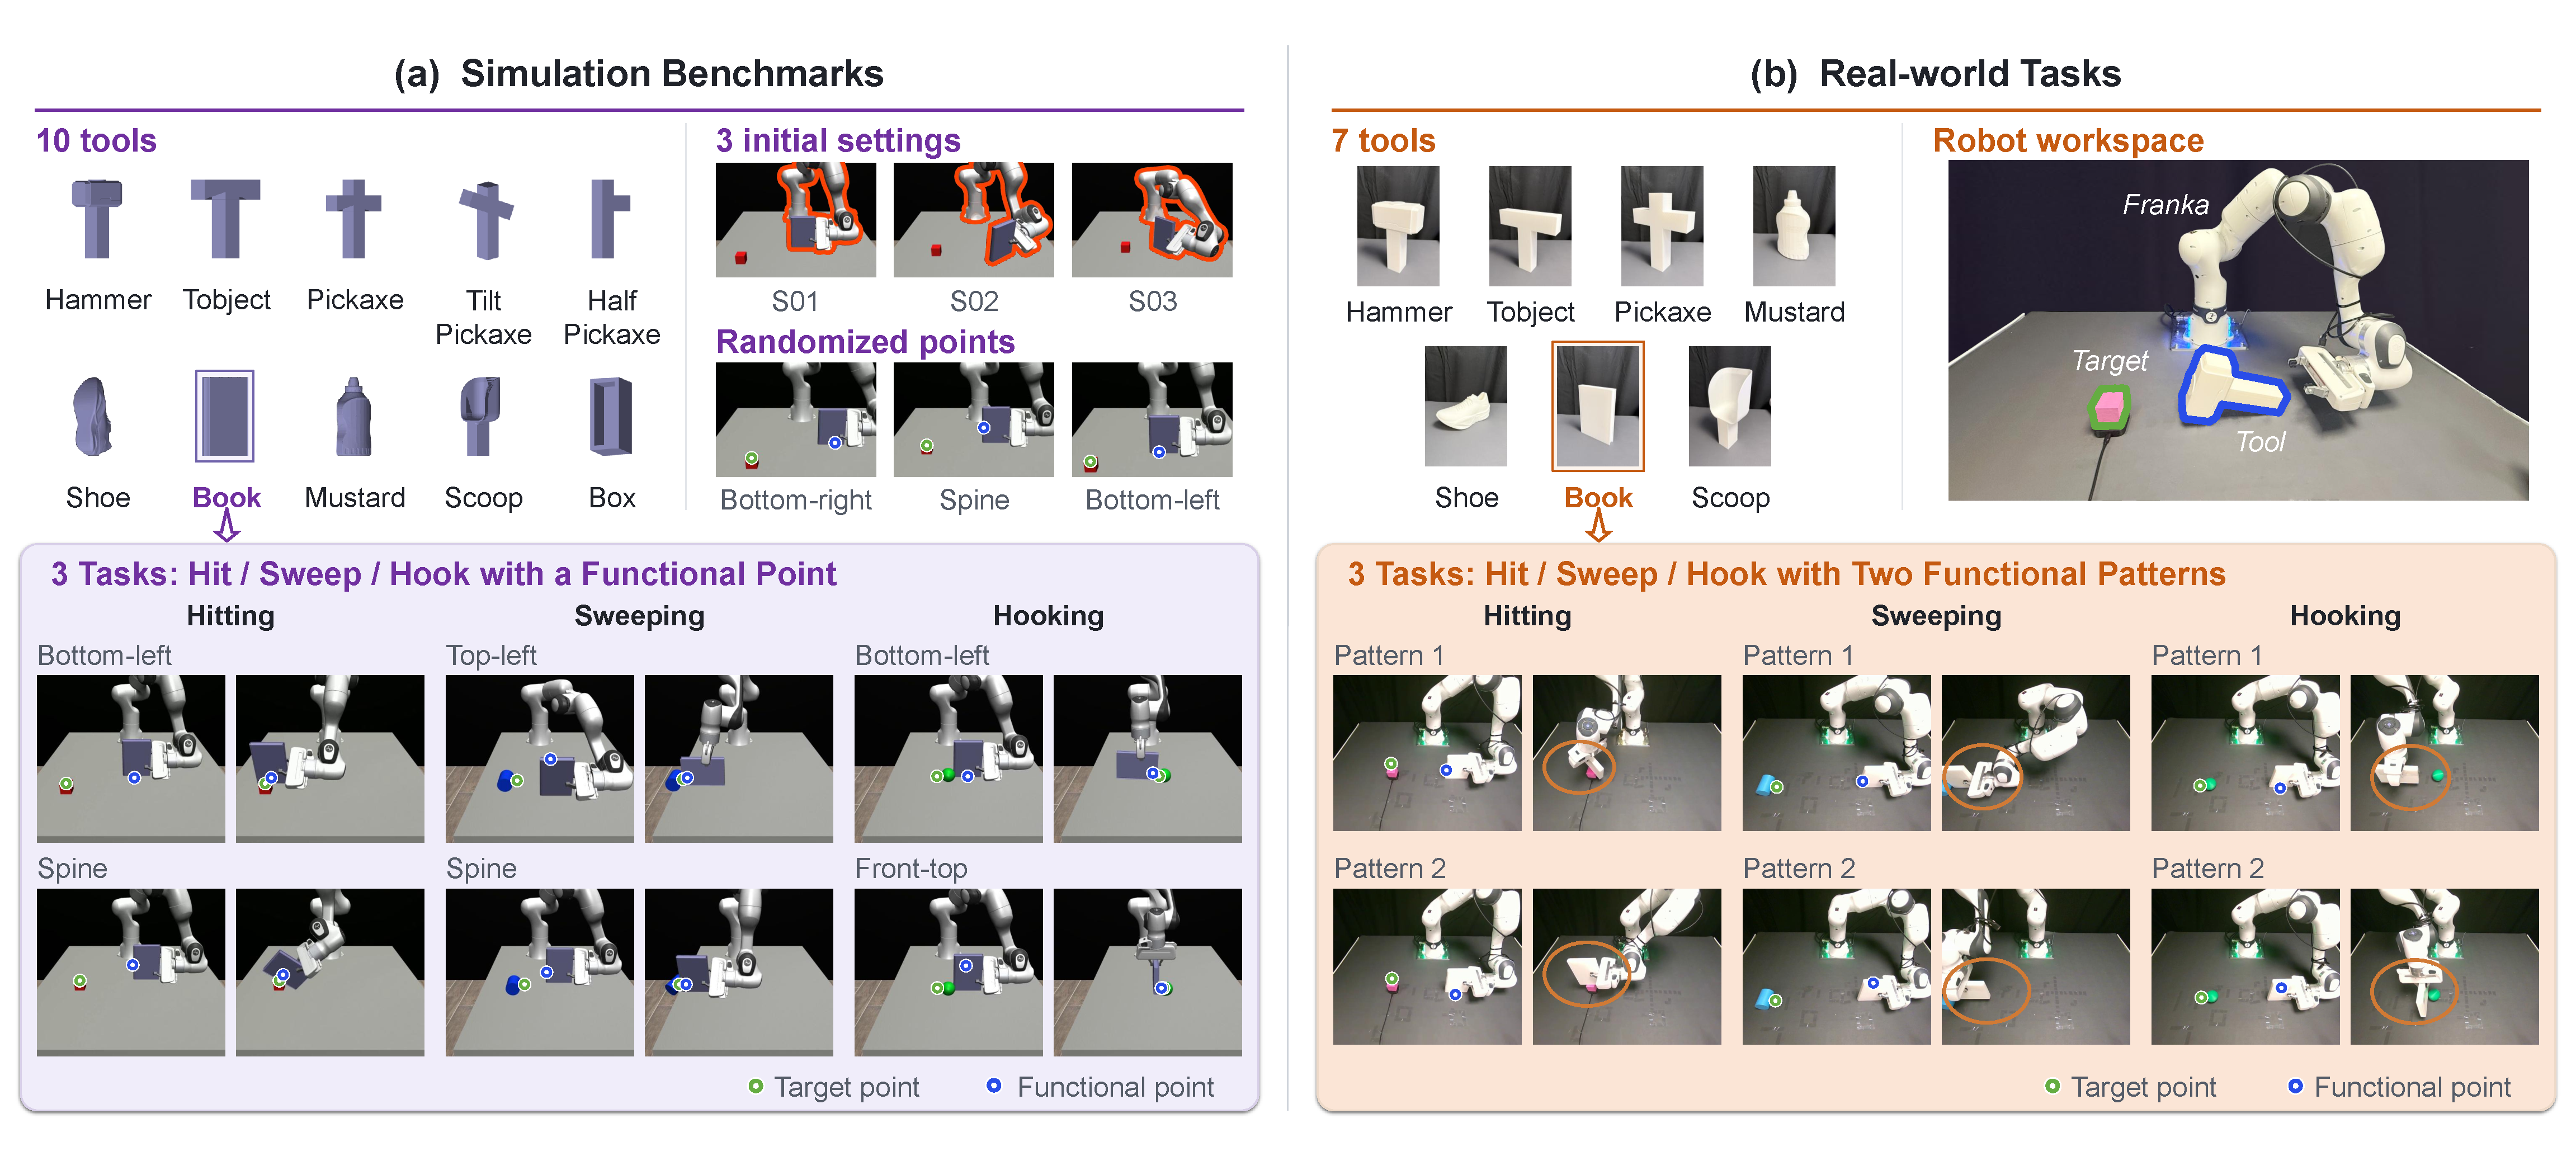
\includegraphics[width=0.95\linewidth]{figures/experiments_settings_v3.pdf}
    \caption{
   \textbf{Simulation Benchmark and Real-World Setting.} (a) The simulation benchmark contains 10 tools and three functions, including hitting, sweeping, and hooking, with multiple initial settings and randomized functional and target points. (b) The real-world benchmark uses a Franka robot with 7 tools and the same three functions, each evaluated under two functional patterns.}
    \label{fig:experiment_settings}
\end{figure}

\vspace{-15pt}
\section{{Experiments}}
\label{sec:experiments}

% highlight真机

Functional generalization remains largely underexplored in robotic manipulation.
In this work, we instantiate it across three representative tool-use functions, including hitting, sweeping, and hooking, and construct both simulation and real-world benchmarks to evaluate whether a policy can transfer each function to unseen tools with diverse geometries.
Specifically, we test four hypotheses underlying the central claims of this work:
% \begin{itemize}[leftmargin=*]
%     \item \textbf{H1}: Functional generalization requires an intermediate representation, not end-to-end mapping.
%     %Tested by the main comparison against FM and DP (Tab.~\ref{tab:simulation_results}).
%     \item \textbf{H2}: Among candidate intermediate representations, 2D keypoint trajectories best balance affordance expressiveness and action groundability.
%     % Tested by the representation ablation (Tab.~\ref{tab:ablation_intermediate_representation}).
%     \item \textbf{H3}: Keypoint trajectories must be function-aware; generic keypoint tracking is not enough.
%     % Tested by the comparison against ATM, which uses pretrained generic keypoints (Tab.~\ref{tab:simulation_results}).
%     \item \textbf{H4}: The two-stage design generalizes under moderate action-labeled tool diversity, making it a practical recipe for tool-use learning.
%     % Tested by the tool-diversity ablation (Tab.~\ref{tab:ablation_tool_generalization_setting}).
% \end{itemize}


\begin{itemize}[leftmargin=*]
    \item \textbf{H1}: Functional generalization benefits from an explicit, function-aware intermediate representation rather than direct perception-to-action mapping or generic motion cues.
    % \item \textbf{H1}: Functional generalization benefits from explicit function-aware motion guidance beyond direct perception-to-action mapping.
    \item \textbf{H2}: Among candidate intermediate representations, 2D keypoint trajectories best balance functional expressiveness and action groundability.
    
    \item \textbf{H3}: Functional generalization can be achieved with moderate action-labeled tool diversity.
    
    \item \textbf{H4}: Functional reasoning is scalable, which can benefit from more diverse action-free data and demonstrate greater autonomy through VLM-based functional point selection.
\end{itemize}


\subsection{Experimental setup}
\label{sec:experiments_setup}
% \textbf{Simulation Benchmark.}~~
% As shown in Fig.~\ref{fig:experiment_settings}, our simulation benchmark contains 7 tools, each with 3 different initial settings. 
% For each tool-setting pair, we collect 30 demonstrations using a four-stage Model Predictive Path Integral (MPPI) planner, resulting in 630 demonstrations in total. The MPPI planner generates an action trajectory by optimizing stage-dependent objectives that sequentially encourage the robot to lift the tool, move it toward the target, align the tool-specific hitting point with the target cube, and execute the final strike. In each demonstration, we randomly initialize the target cube position and sample the tool-specific hitting point along the tool boundary, requiring the policy to adapt its motion to both the tool geometry and the target location. In the main setting, all methods are trained on 4 tools, including hammer, tobject, pickaxe, and mustard, and evaluated on the remaining 3 unseen tools. During evaluation, each unseen tool is tested under three initial settings with 30 rollout episodes. A rollout is considered successful only if the robot strikes the target cube using the designated hitting point.

% \textbf{Simulation Benchmark.}~~As shown in Fig.~\ref{fig:experiment_settings}, our simulation benchmark contains 10 tools and three tool-use functions, including hitting, sweeping, and hooking, with three initial settings for each tool. 
% For each tool-setting-function combination, we collect 30 demonstrations using MPPI-based planners with function-specific objectives, resulting in 2,700 demonstrations in total. 
% In each demonstration, we randomize the target position and the tool-specific functional point, requiring the policy to adapt its motion to the tool geometry, functional point, and target configuration.
% In the main setting, all grounded execution policies are trained with action-labeled data
% from four seen tools, including hammer, tobject, pickaxe, and mustard, and evaluated on three unseen tools, including scoop, shoe, and book, across all three functions.
% During evaluation, each unseen tool is tested under three initial settings with 30 rollout episodes per setting.
% A rollout is considered successful only if the specified function is completed using the designated functional point: for \textit{hitting}, the selected hitting point must strike the red cube; for \textit{sweeping}, the selected sweeping point must push the blue cylinder; and for \textit{hooking}, the selected hooking point must hook the green ball inward. For the same tool and function, different functional points may be specified, e.g., using either the hammer head or handle for hitting.


\textbf{Simulation Benchmark.}~~
As shown in Fig.~\ref{fig:experiment_settings}, our simulation benchmark covers 10 tools and three functions, including hitting, sweeping, and hooking, with three initial settings per tool.
For each tool-setting-function combination, we collect 30 demonstrations using function-specific MPPI planners, totaling 2,700 demonstrations.
In the main setting, all methods are trained on action-labeled data from four tools (hammer, tobject, pickaxe, and mustard) and evaluated on three unseen tools held out from action-labeled training (scoop, shoe, and book) across all functions.
% In the main setting, all grounded execution policies are trained on action-labeled data from four seen tools (hammer, tobject, pickaxe, and mustard) and evaluated on three unseen tools (scoop, shoe, and book) across all functions.
Each unseen tool is evaluated under three initial settings with 30 rollouts per setting.
For each demonstration, we randomize the target position and designated functional point, with different points possible for the same tool and function (e.g., using the hammer head or handle for hitting).
A rollout is successful only if the specified function is completed using that point: \textit{hitting} requires the hitting point to strike the red cube, \textit{sweeping} requires the sweeping point to push the blue cylinder, and \textit{hooking} requires the hooking point to pull the green ball inward.




% \textbf{Real-World Setting.}~~
% We further construct a real-world benchmark on a Franka robot platform, as shown in Fig.~\ref{fig:experiment_settings}. 
% The real-world setting contains 3 tools: hammer, mustard, and book. 
% Each tool has two hitting patterns, and each pattern contains 20 expert demonstrations, resulting in 120 real-world trajectories.
% We train the policy on hammer and mustard and evaluate its functional generalization ability on the unseen book tool. 
% For each hitting pattern, we perform 20 real-world rollout trials. A trial is successful if the robot follows the specified hitting pattern and strikes the target.

% \textbf{Real-World Setting.}~~
% We further construct a real-world benchmark on a Franka robot platform, as shown in Fig.~\ref{fig:experiment_settings}.
% The benchmark covers 7 tools and the same three functions, with two functional patterns defined for each function.
% For each training tool and functional pattern, we collect 20 expert demonstrations.
% For hitting, we train the policies on hammer, pickaxe, and mustard and evaluate on three unseen tools: tobject, book, and shoe.
% For sweeping and hooking, we train the policies on hammer and mustard and evaluate on the unseen book.
% Each pattern is evaluated with 10 real-world rollout trials, and a trial is considered successful if the robot completes the specified function using the designated functional point.


\textbf{Real-World Setting.}~~
We further construct a real-world benchmark on a Franka robot platform.
The benchmark covers 7 tools and the same three functions, with two functional patterns defined for each function.
For each training tool and functional pattern, we collect 20 expert demonstrations.
For hitting, the policies are trained on hammer, pickaxe, and mustard and evaluated on three unseen tools (tobject, book, and shoe).
For sweeping and hooking, they are trained on hammer and mustard and evaluated on the unseen book.
Each functional pattern is evaluated with 10 real-world rollouts.
Unlike simulation, the designated functional point specifies the required functional pattern rather than serving as a point-level success criterion. A rollout is successful if the robot completes the specified function following the corresponding pattern.


% \textbf{Baselines.}~~We compare \algoname{} against three baselines covering end-to-end and keypoint-based policies. All baselines receive the same inputs as \algoname{}: visual observations, proprioceptive states, and the initial functional and target point positions. \textit{Flow-Matching (FM)}~\citep{lipmanflow} and \textit{Diffusion Policy (DP)}~\citep{chi2025diffusion} are end-to-end visuomotor policies that map observations directly to actions, serving as references for the perception-to-action gap (Sec.~\ref{sec:intro}). \textit{ATM}~\citep{wen2023any} also conditions on keypoint trajectories, but obtains them from a generic tracker pretrained on LIBERO-90 rather than a function-aware predictor, allowing us to test whether the gain comes from using keypoints or from predicting function-aware keypoint motion.

\textbf{Baselines.}~~
We compare \algoname{} against three baselines covering end-to-end and keypoint-based policies.
All baselines receive the same inputs as \algoname{}: visual observations, proprioceptive states, and the initial functional, target, and tool point positions.
\textit{Flow-Matching (FM)}~\citep{lipmanflow} and \textit{Diffusion Policy (DP)}~\citep{chi2025diffusion} are end-to-end visuomotor policies that map observations directly to actions, serving as references for the perception-to-action gap (Sec.~\ref{sec:intro}).
\textit{ATM}~\citep{wen2023any} conditions the execution policy on keypoint trajectories. Given the functional and target points, it uses its generic any-point trajectory model pretrained on LIBERO-90 to predict their trajectories. This serves as a keypoint-based baseline using generic trajectory modeling rather than explicitly predicting function-aware keypoint motion.


\textbf{Evaluation Metrics.}~~
All experiments report the success rate (SR) as the main evaluation metric, which is defined as the number of successful trials divided by the total number of rollout trials.


\begin{table}[ht]
\centering
\caption{\textbf{Simulation Results on Unseen Tools.} Success rate (SR) on three unseen tools across hitting, sweeping, and hooking. Each tool is evaluated under 3 settings with 30 rollouts per setting.}
\label{tab:simulation_results}
\small
\setlength{\tabcolsep}{3.0pt}

\resizebox{0.9\linewidth}{!}{
\begin{tabular}{lcccccccccccc}
\toprule
& \multicolumn{4}{c}{Hitting} 
& \multicolumn{4}{c}{Sweeping}
& \multicolumn{4}{c}{Hooking} \\
\cmidrule(lr){2-5}
\cmidrule(lr){6-9}
\cmidrule(lr){10-13}

Method 
& Scoop & Shoe & Book & Avg. 
& Scoop & Shoe & Book & Avg.
& Scoop & Shoe & Book & Avg. \\
\midrule

FM 
& 0.07 & 0.03 & 0.16 & \cellcolor{gray!15} 0.09 
& 0.49 & 0.23 & 0.19 & \cellcolor{gray!15} 0.30
& 0.22 & 0.06 & 0.14 & \cellcolor{gray!15} 0.14 \\

DP 
& 0.18 & 0.08 & 0.26 & \cellcolor{gray!15} 0.17 
& 0.49 & 0.18 & 0.13 & \cellcolor{gray!15} 0.27
& 0.12 & 0.06 & 0.08 & \cellcolor{gray!15} 0.09 \\

ATM 
& 0.12 & 0.06 & 0.06 & \cellcolor{gray!15} 0.08 
& 0.41 & 0.16 & 0.19 & \cellcolor{gray!15} 0.25
& 0.10 & 0.07 & 0.24 & \cellcolor{gray!15} 0.14 \\

\midrule

\algoname{} 
& \textbf{0.42} & \textbf{0.23} & \textbf{0.42} 
& \cellcolor{gray!15}\textbf{0.36} 
& \textbf{0.71} & \textbf{0.29} & \textbf{0.34} 
& \cellcolor{gray!15}\textbf{0.45}
& \textbf{0.29} & \textbf{0.17} & \textbf{0.24} 
& \cellcolor{gray!15}\textbf{0.23} \\

\bottomrule
\end{tabular}
}
\end{table}



\begin{table}[ht]
\centering
% \caption{\textbf{Real-world evaluation on unseen tools across different functions.}
% For hitting, the policy is trained on hammer, pickaxe, and mustard and evaluated on three unseen tools.
% For sweeping and hooking, the policy is evaluated on the unseen book under two configurations.}
\caption{\textbf{Real-World Results on Unseen Tools.} Success rate (SR) under two functional patterns for hitting, sweeping, and hooking. Hitting is evaluated on three unseen tools, while sweeping and hooking are evaluated on the unseen book, with 10 rollouts per pattern.}

\label{tab:real_world_results}
\small
\setlength{\tabcolsep}{2.0pt}

\resizebox{0.9\linewidth}{!}{
\begin{tabular}{lccccccccccccccc}
\toprule
& \multicolumn{9}{c}{\textbf{Hitting}}
& \multicolumn{3}{c}{\textbf{Sweeping}}
& \multicolumn{3}{c}{\textbf{Hooking}} \\
\cmidrule(lr){2-10}
\cmidrule(lr){11-13}
\cmidrule(lr){14-16}

& \multicolumn{3}{c}{Tobject}
& \multicolumn{3}{c}{Book}
& \multicolumn{3}{c}{Shoe}
& \multicolumn{3}{c}{Book}
& \multicolumn{3}{c}{Book} \\
\cmidrule(lr){2-4}
\cmidrule(lr){5-7}
\cmidrule(lr){8-10}
\cmidrule(lr){11-13}
\cmidrule(lr){14-16}

Method
& P01 & P02 & Avg.
& P01 & P02 & Avg.
& P01 & P02 & Avg.
& P01 & P02 & Avg.
& P01 & P02 & Avg. \\
\midrule

FM
& 0.00 & 0.60 & \cellcolor{gray!15} 0.30
& 0.50 & 0.00 & \cellcolor{gray!15} 0.25
& 0.00 & 0.20 & \cellcolor{gray!15} 0.10
& 0.30 & 0.00 & \cellcolor{gray!15} 0.15
& 0.20 & 0.00 & \cellcolor{gray!15} 0.10 \\

\algoname{}
& \textbf{0.60} & \textbf{0.80} & \cellcolor{gray!15}\textbf{0.70}
& \textbf{0.60} & \textbf{1.00} & \cellcolor{gray!15}\textbf{0.80}
& \textbf{0.20} & \textbf{0.60} & \cellcolor{gray!15}\textbf{0.40}
& \textbf{0.80} & \textbf{0.30} & \cellcolor{gray!15}\textbf{0.55}
& \textbf{0.90} & \textbf{0.30} & \cellcolor{gray!15}\textbf{0.60} \\

\bottomrule
\end{tabular}
}

\end{table}




\subsection{Main Results \& Analysis}

\textbf{Simulation Results.}~~
% As shown in Tab.~\ref{tab:simulation_results}, \algoname{} outperforms all baselines across hitting, sweeping, and hooking on unseen tools.
% Compared with the best baseline results of $0.17$, $0.30$, and $0.14$, it achieves average SRs of $0.36$, $0.45$, and $0.23$, respectively.
% The weak performance of FM and DP suggests that direct perception-to-action mapping struggles to adapt tool-specific motions to unseen geometries without tool-specific action supervision, while ATM shows that generic keypoint trajectories alone are insufficient to provide function-relevant motion guidance.
% Together, these results support \textbf{H1}: functional generalization benefits from an explicit, function-aware intermediate representation.
As shown in Tab.~\ref{tab:simulation_results}, \algoname{} outperforms all baselines across hitting, sweeping, and hooking on unseen tools.
Compared with the best baseline results of $0.17$, $0.30$, and $0.14$, it achieves average SRs of $0.36$, $0.45$, and $0.23$, respectively.
The weak performance of FM and DP suggests that direct perception-to-action mapping struggles to adapt tool-specific motions to unseen geometries without tool-specific action supervision.
Despite being conditioned on the designated functional and target points, ATM performs less effectively, suggesting that its generic keypoint predictor may fail to produce effective function-relevant motion guidance for diverse tool geometries.
Together, these results support \textbf{H1}: explicit function-aware intermediate representation provides useful guidance for functional generalization.


\textbf{Real-World Results.}~~
We test \algoname{} on the real-world benchmark across all three functions.
As shown in Tab.~\ref{tab:real_world_results}, \algoname{} consistently outperforms the FM baseline across all evaluated unseen-tool and functional-pattern settings. These results extend the evidence for \textbf{H1} to real-world manipulation, showing that function-aware keypoint plans provide more reliable guidance.
% For hitting, \algoname{} achieves average SRs of $0.70$, $0.80$, and $0.40$ on tobject, book, and shoe, compared with $0.30$, $0.25$, and $0.10$ for FM.
% On the unseen book, it further improves the average SR from $0.15$ to $0.55$ for sweeping and from $0.10$ to $0.60$ for hooking.
% These results extend the evidence for \textbf{H1} to real-world manipulation, showing that function-aware keypoint plans provide more reliable guidance.
%than direct perception-to-action mapping across diverse functions and unseen tools.

\textbf{Failure Case Analysis.}~~
We further examine representative baseline failures on the hitting function in both simulation and the real world.
As shown in Fig.~\ref{fig:qualitative-analysis}, the baselines exhibit three typical failure modes: \emph{pass over}, where the tool moves across the target without establishing the intended contact; \emph{imprecise hitting}, caused by insufficient fine-grained spatial alignment; and \emph{tool dropping}, associated with unstable or overly aggressive motions.
In the corresponding cases, \algoname{} successfully completes the task by predicting function-aware keypoint trajectories that guide the functional region toward the target with the appropriate motion and alignment.
Additional qualitative comparisons across hitting, sweeping, and hooking in both simulation and the real world are provided in App.~\ref{app:additional_experimental_results}.


\begin{figure}[ht]
    \centering
    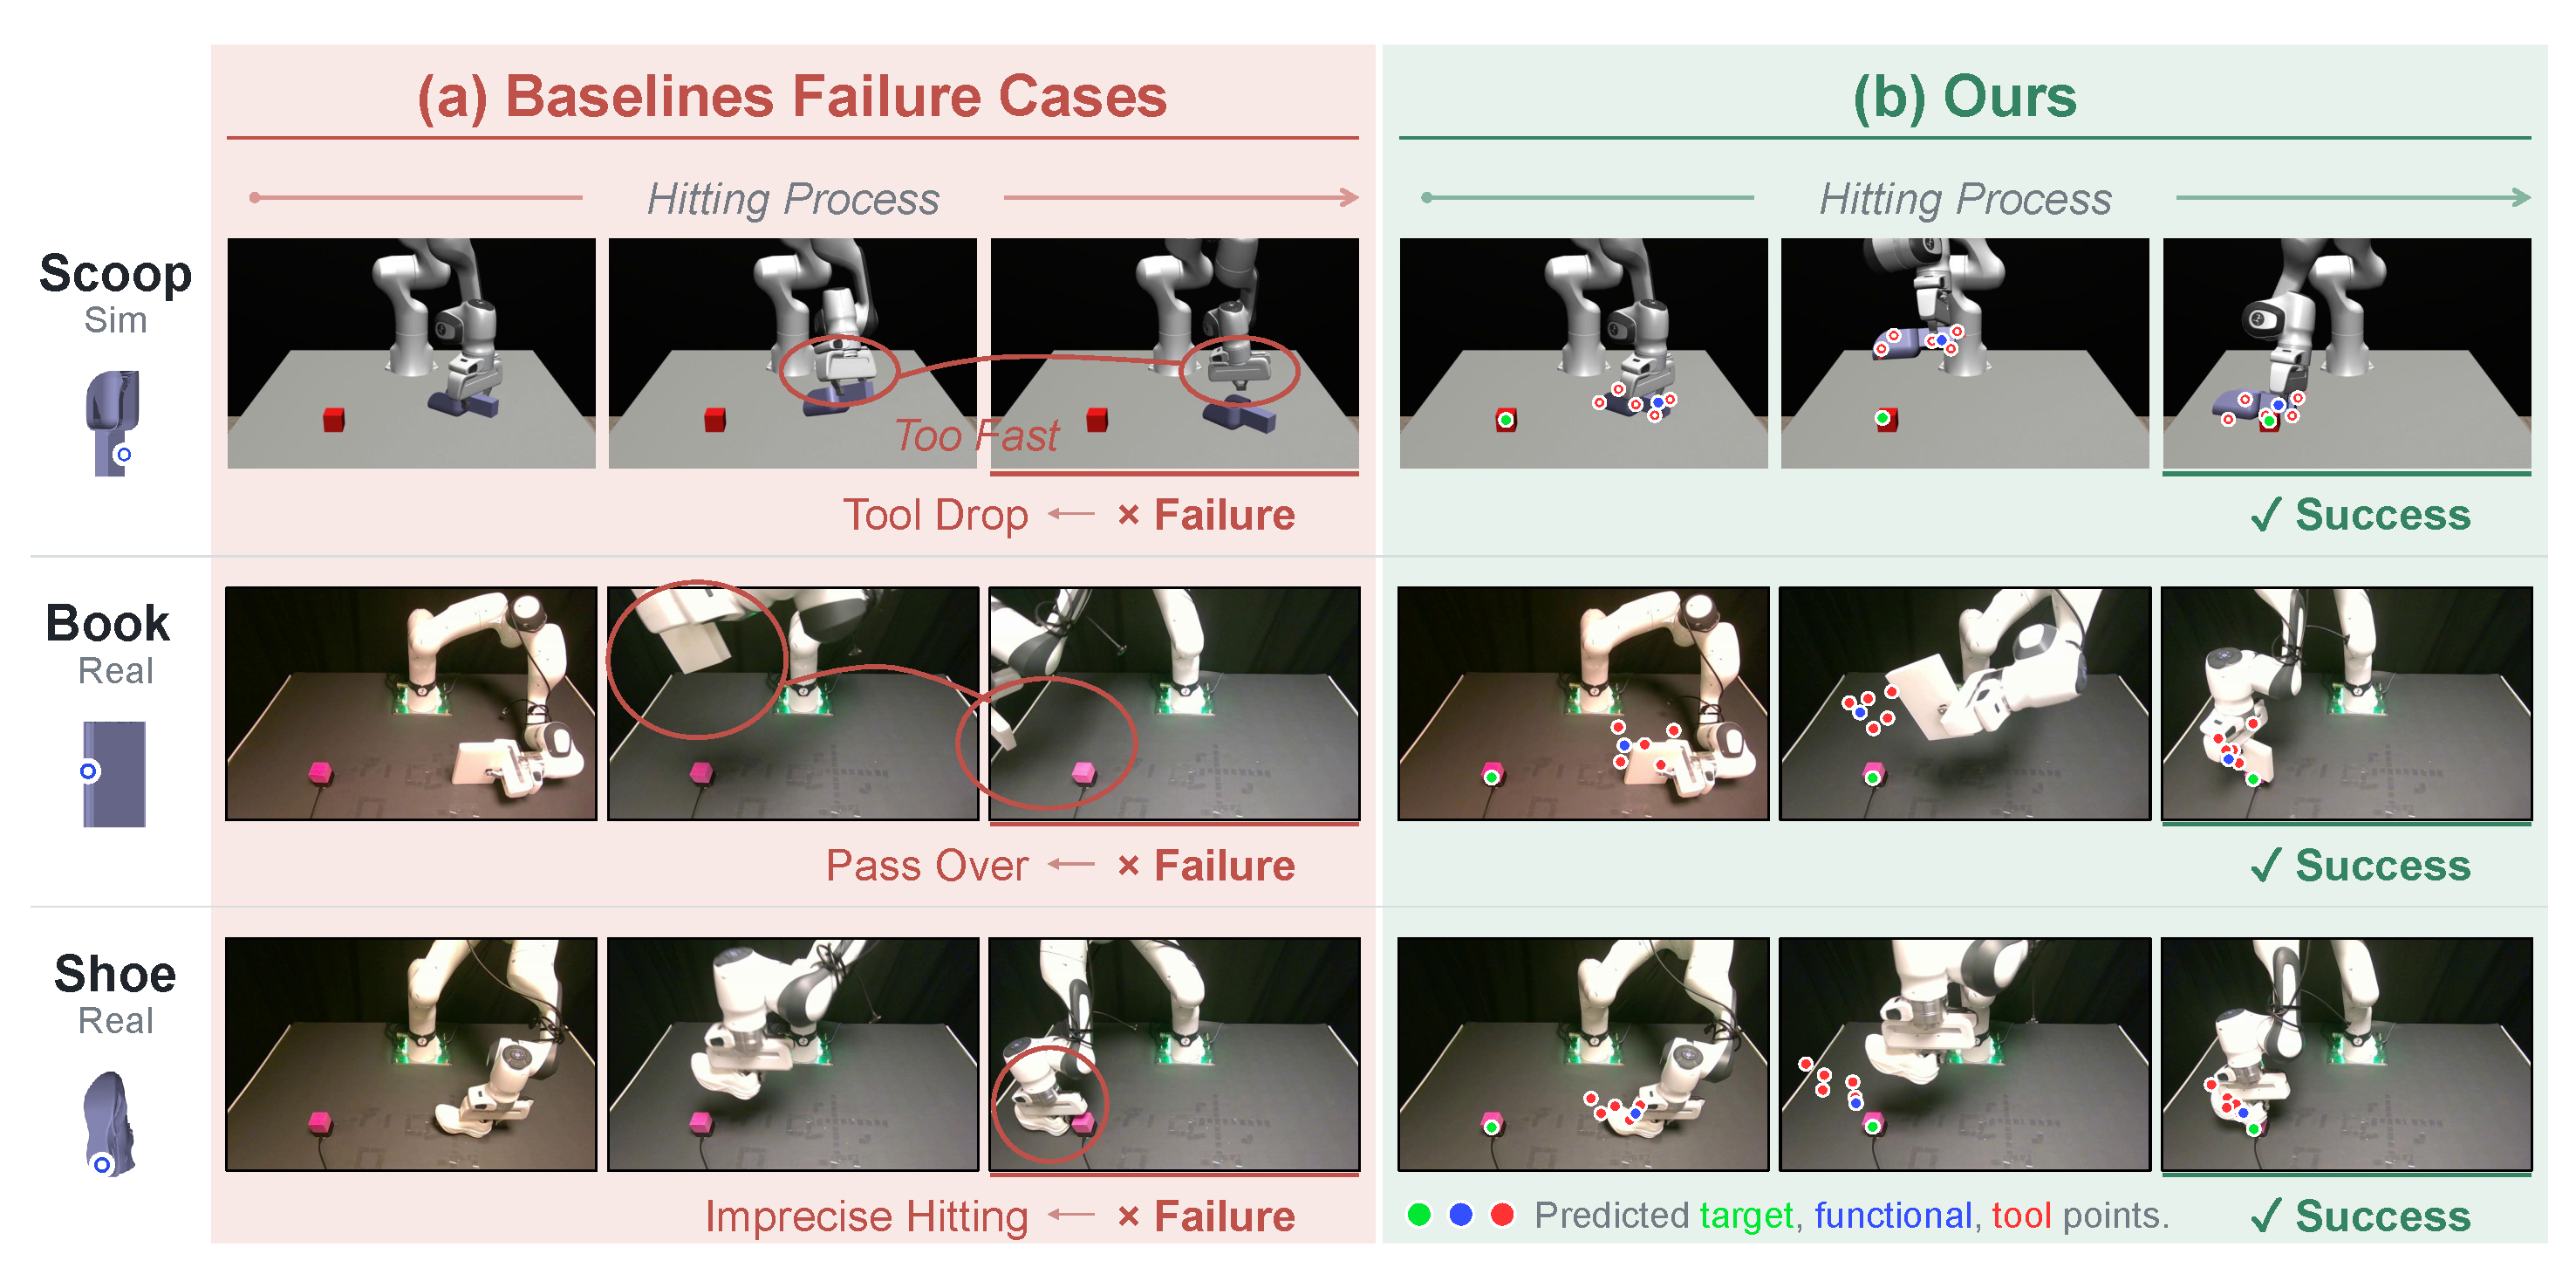
\includegraphics[width=0.82\linewidth]{figures/qualitative_results_v2.pdf}
    \caption{\textbf{Qualitative Comparison on Unseen Tools.} Representative baseline failure cases and successful rollouts of \algoname{} for hitting in simulation and the real world.}

    \label{fig:qualitative-analysis}
\end{figure}


\subsection{Ablation Studies}
% Beyond the main comparisons, we conduct two ablations to dissect the key design choices behind \algoname{}.
% Unless otherwise specified, all ablation experiments are conducted on the hitting function in simulation.
% First, we vary the functional intermediate representation while keeping the execution policy fixed, comparing affordance images, human video prompts, per-frame functional videos and object masks, and 2D keypoint trajectories to assess which representation best balances functional expressiveness and action groundability.
% The second ablation varies the diversity of action-labeled tools, training \algoname{} on 1, 4, or 7 tools and testing on the three unseen tools, to evaluate whether the two-stage design provides a practical recipe for functional generalization using moderate robotic data.
Beyond the main comparisons, we conduct two ablations on the key design choices of \algoname{}: the functional intermediate representation and the diversity of action-labeled tools.
Unless otherwise specified, all ablations are conducted on the hitting function in simulation.


\subsubsection{Effect of Functional Intermediate Representations.}

\begin{table}[ht]
\centering
\caption{\textbf{Ablation Results on Functional Intermediate Representations.} Success rate (SR) for hitting on unseen tools when different representations condition the same execution policy $\pi_{\mathrm{sys1}}$.}
\label{tab:ablation_intermediate_representation}
\small

\begin{tabular*}{0.9\linewidth}{
@{\extracolsep{\fill}}
llccc>{\columncolor{gray!12}}c
}
\toprule
Representation & Temporal input & Scoop & Shoe & Book & \cellcolor{white}Avg. \\
\midrule
None (FM) & -- & 0.07 & 0.03 & 0.16 & 0.09 \\
Affordance image & Static & 0.34 & 0.11 & 0.16 & 0.20 \\
Human video prompt & Pooled & 0.26 & 0.09 & 0.23 & 0.19 \\
\midrule
Per-frame video & Sequence & 0.28 & 0.13 & 0.29 & 0.23 \\
Per-frame object masks & Sequence & 0.37 & 0.16 & 0.43 & 0.32 \\
Keypoint trajectories & Sequence &
\textbf{0.50} & \textbf{0.31} & \textbf{0.67} & \textbf{0.49} \\
\bottomrule
\end{tabular*}

\end{table}

As discussed in Sec.~\ref{sec:Functional Intermediate Representations Selection}, we investigate the effect of functional intermediate representations by training and evaluating the execution policy $\pi_{\mathrm{sys1}}$ with pre-extracted representations as conditions.
Results in Tab.~\ref{tab:ablation_intermediate_representation} show that static affordance images and pooled human video prompts improve generalization, indicating that functional-region cues and motion demonstrations provide guidance.
Providing temporally varying representations improves performance, while object masks achieve stronger generalization by only retaining object-centric motion cues.
Among representations, 2D keypoint trajectories perform best, as they compactly encode fine-grained functional and target locations together with their structured motion over time.
These results support \textbf{H2}: keypoint trajectories best balance functional expressiveness and action groundability.



\subsubsection{Effect of Action-Labeled Tool Diversity.}
\begin{wraptable}{r}{0.54\linewidth}
\vspace{-0.8em}
\centering
\captionsetup{skip=4pt}
\caption{\textbf{Ablation on Action-Labeled Tool Diversity.} Success rate (SR) of \algoname{} when the execution policy $\pi_{\mathrm{sys1}}$ is trained with action-labeled data from $M=1 \text{,} 4 \text{,} 7$ tools and consistently evaluated on the same three unseen tools: scoop, shoe, and book.}
\label{tab:ablation_tool_generalization_setting}

\resizebox{0.95\linewidth}{!}{
\begin{tabular}{lcccc}
\toprule
\multirow{2}{*}{Method}
& \multicolumn{4}{c}{Tools} \\
\cmidrule(lr){2-5}
& Scoop & Shoe & Book & Avg. \\
\midrule
\algoname{} (1-to-3) & 0.14 & 0.10 & 0.23 & \cellcolor{gray!12} 0.16 \\
\algoname{} (4-to-3) & 0.42 & 0.23 & 0.42 & \cellcolor{gray!12} 0.36 \\
\algoname{} (7-to-3) & 0.39 & 0.27 & 0.52 & \cellcolor{gray!12} 0.39 \\
\bottomrule
\end{tabular}
}
\vspace{-0.8em}
\end{wraptable}
% Beyond the standard 4-to-3 setting, we vary the number of action-labeled training tools, while consistently evaluating on the same three unseen tools: scoop, shoe, and book.
% As shown in Tab.~\ref{tab:ablation_tool_generalization_setting}, increasing the training diversity from 1 to 4 tools substantially improves the average success rate from $0.16$ to $0.36$, while further increasing it to 7 tools yields only a marginal gain to $0.39$.
% This saturation is consistent with the role of System-1, which primarily grounds functional plans into executable actions rather than learning cross-tool functional reasoning. Therefore, moderate robotic data already provides sufficient coverage for action grounding, suggesting that further performance improvements increasingly depend on improving the System-2 functional planner.
% These results support \textbf{H3}: moderate action-labeled robotic data is sufficient to support functional generalization in our two-stage framework.
Beyond the standard 4-to-3 setting, we vary the number of action-labeled training tools while consistently evaluating on the same three unseen tools: scoop, shoe, and book.
As shown in Tab.~\ref{tab:ablation_tool_generalization_setting}, increasing the training diversity from 1 to 4 tools substantially improves the average SR from $0.16$ to $0.36$, while further increasing it to 7 tools yields a smaller gain to $0.39$.
These results support \textbf{H3}: functional generalization can be achieved with moderate action-labeled tool diversity in our two-stage framework.


% figure 5的文字放大一些。
\begin{figure}[ht]
    \centering
    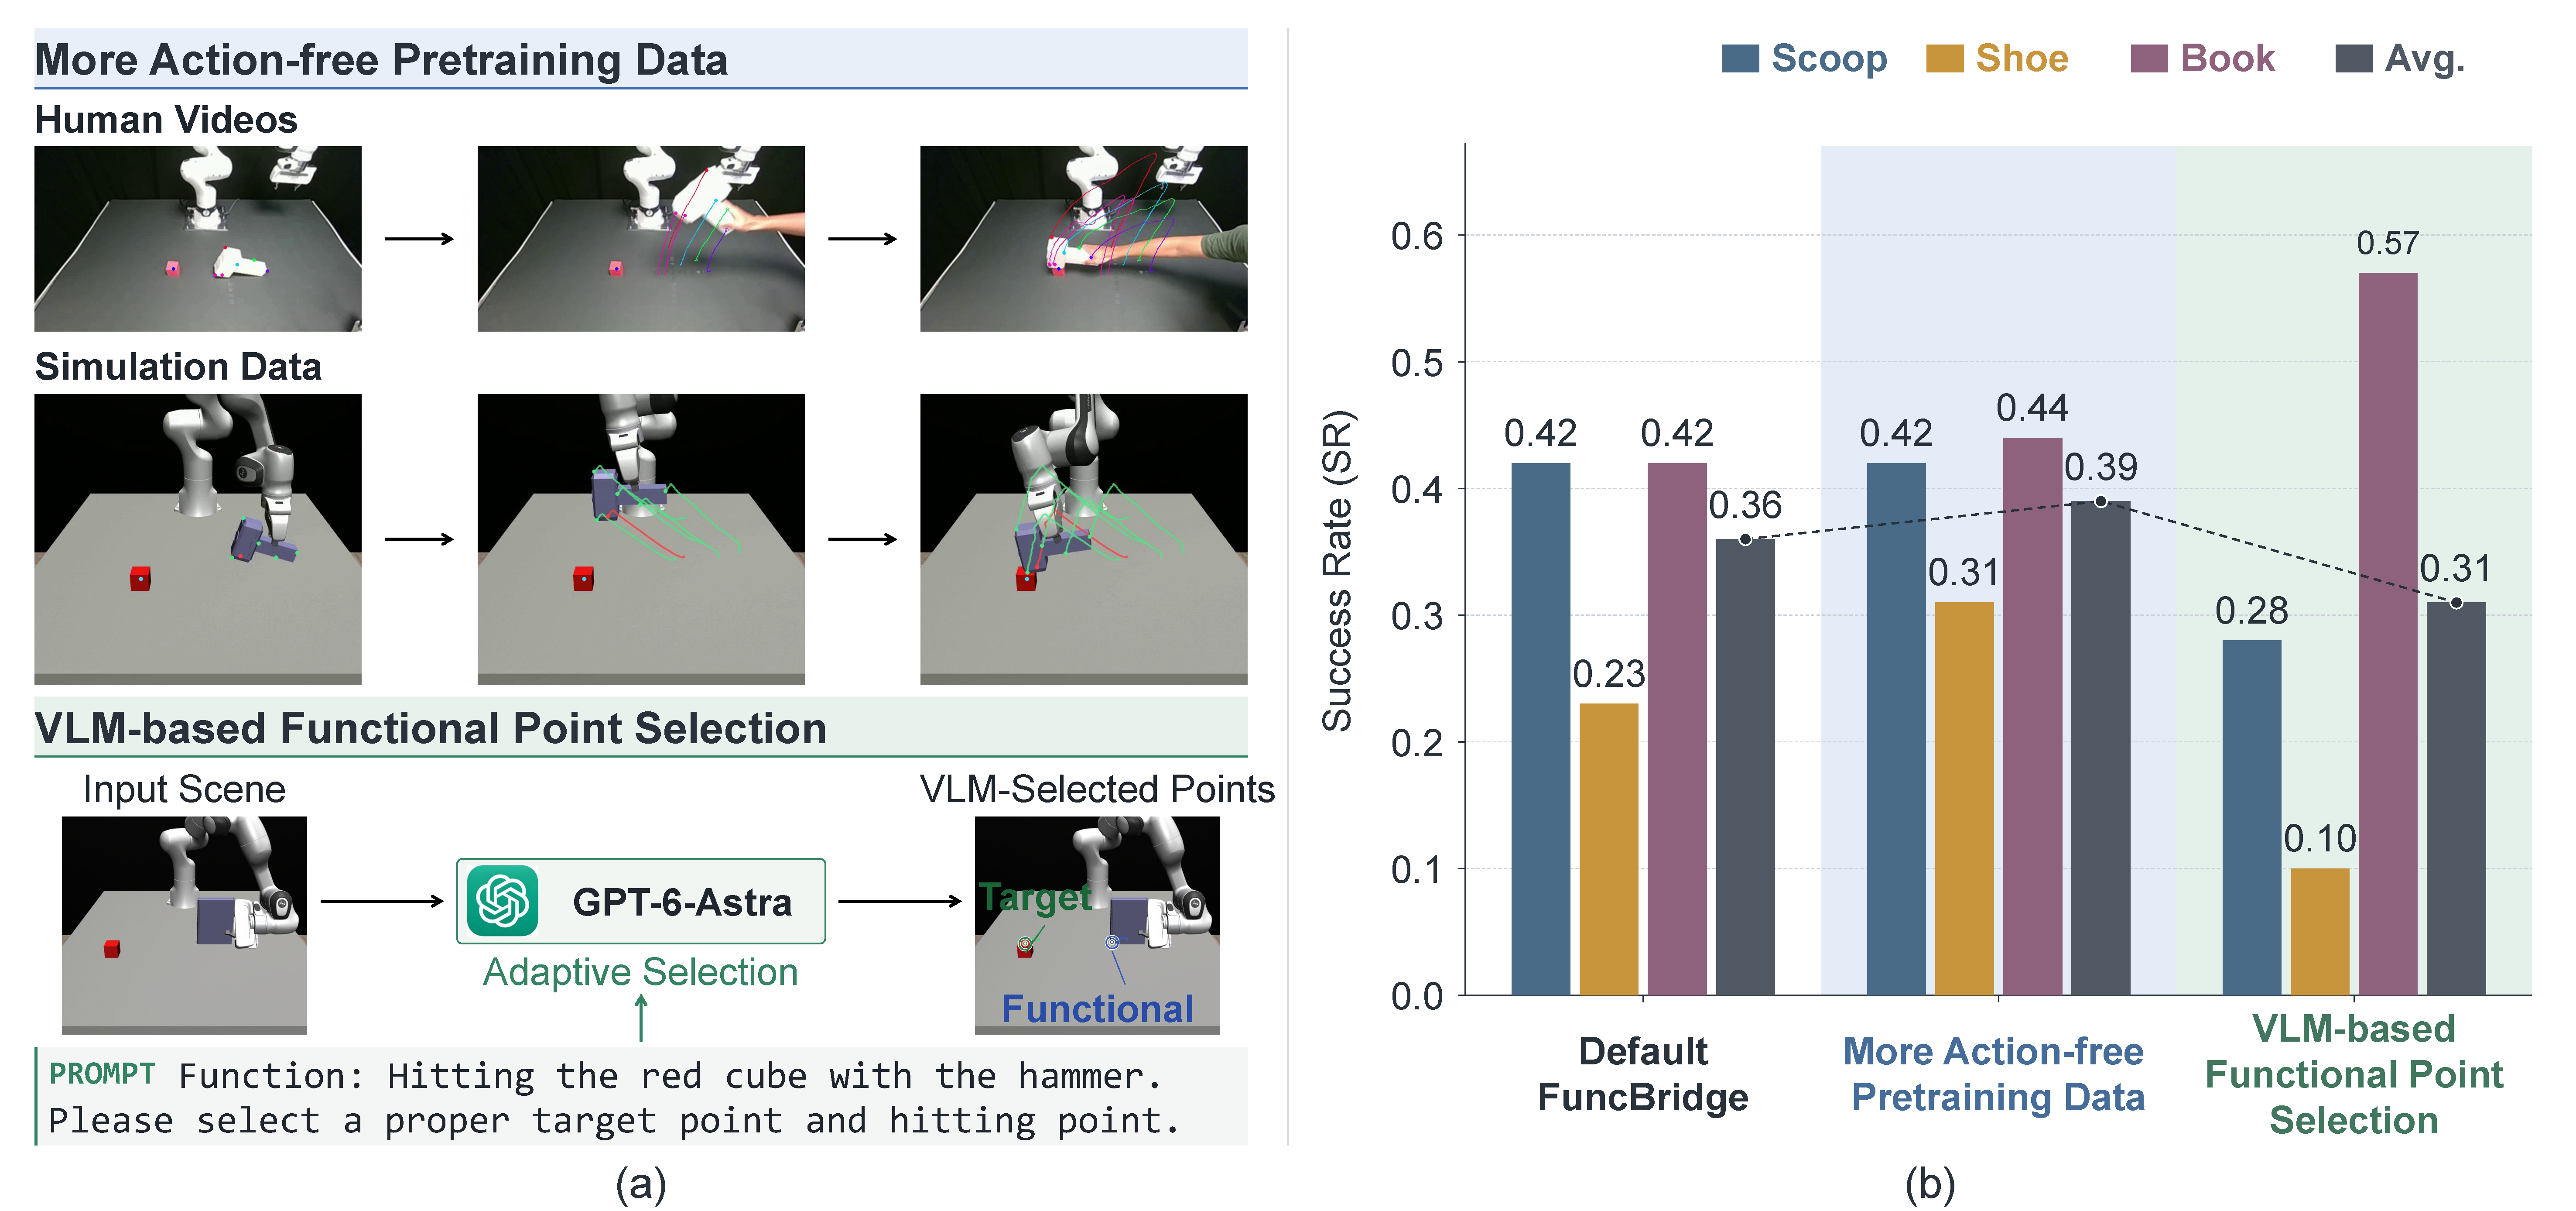
\includegraphics[width=0.95\linewidth]{figures/further_analysis_v2.pdf}
    \caption{\textbf{Scalability of \algoname{}.} (a) Extensions using human videos and VLM-based functional point selection. (b) Success rates on unseen tools for the default model and each extension.}

    \label{fig:further-analysis}
\end{figure}


% \subsection{Scalability of \algoname{}}
% \label{sec:scalability}

% Our default setting learns functional reasoning from action-free simulation videos and uses provided functional and target points at evaluation. We test \textbf{H4} through human-video pretraining and VLM-based point selection.

% \subsubsection{Scaling Action-Free Pretraining with Human Videos.}
% \label{sec:scalability-human-video}
% We augment the action-free pretraining data for $\pi_{\mathrm{sys2}}$ with 525 keypoint-annotated human hitting videos (App.~\ref{app:fir_extraction}), keeping the same four-tool action-labeled data for fine-tuning $\pi_{\mathrm{sys1}}$. Average SR increases from $0.36$ to $0.39$ (Fig.~\ref{fig:further-analysis}), showing that \algoname{} benefits from heterogeneous action-free data.

% \subsubsection{Flexible VLM-Based Functional Point Selection.}
% Given the observed scene and task instruction, GPT-6-Astra selects the tool's functional point and the target point for \algoname{}'s planning and execution. VLM-selected points achieve an average SR of $0.31$, versus $0.36$ with manually specified points (Fig.~\ref{fig:further-analysis}), supporting more autonomous tool use without manual point specification.

\subsection{Scalability of \algoname{}}
\label{sec:scalability}

Our default setting learns functional reasoning from action-free simulation videos, while the functional and target points are provided during evaluation.
We further examine \textbf{H4} by extending \algoname{} with multi-source action-free data and VLM-based function-relevant point selection.
% Our default setting learns functional reasoning from action-free tool-use videos collected within the simulation benchmark, while the functional and target points are provided during evaluation. We further examine whether \algoname{} can scale beyond these settings by leveraging multi-sourced action-free data and automatically identifying function-relevant points with a VLM agent. Together, these analyses support \textbf{H4}.
% Our default setting learns functional reasoning from action-free simulation videos, with functional and target points provided at evaluation.
% We further examine \textbf{H4} using multi-source action-free data and VLM-based point selection.

\subsubsection{Scaling Action-Free Pretraining with Human Videos.}
\label{sec:scalability-human-video}
As shown in Fig.~\ref{fig:further-analysis} (a), we additionally collect and annotate keypoints of 525 human videos for the hitting function (see App.~\ref{app:fir_extraction} for details).
Together with the original action-free data, these videos are used to pretrain $\pi_{\mathrm{sys2}}$, while $\pi_{\mathrm{sys1}}$ is fine-tuned with the same four-tool action-labeled robotic data.
As shown in Fig.~\ref{fig:further-analysis} (b), incorporating human videos improves the average SR from $0.36$ to $0.39$.
This result shows that \algoname{} can benefit from heterogeneous action-free data, suggesting the potential of broader data sources for functional reasoning.

\subsubsection{Flexible VLM-Based Functional Point Selection.}
% We further reduce the reliance on manually provided functional and target points by introducing a VLM agent.
% Given the observed scene and task instruction, GPT-6-Astra is prompted to adaptively select the functional point on the tool and the target point, which are then used by \algoname{} for functional planning and grounded execution.
% As shown in Fig.~\ref{fig:further-analysis}, VLM-selected points achieve an average SR of $0.31$, compared with $0.36$ using manually specified points.
% The relatively small performance gap suggests that the generalization capability of VLMs can be naturally combined with \algoname{} to enable more autonomous functional tool use without manually specifying function-relevant points.
% Given the observed scene and task instruction, GPT-6-Astra is prompted to adaptively select the functional point on the tool and the target point, which are then used by \algoname{} for functional planning and grounded execution.
% As shown in Fig.~\ref{fig:further-analysis}, VLM-selected points achieve an average SR of $0.31$, compared with $0.36$ using manually specified points.
% The relatively small performance gap suggests that the generalization capability of VLMs can be combined with \algoname{} to enable more autonomous functional tool use without manually specifying function-relevant points.
Given the observed scene and task instruction, GPT-6-Astra is prompted to adaptively select the functional point on the tool and the target point, which are then used by \algoname{} for functional planning and grounded execution.
A rollout is considered successful if the VLM-selected functional point is used to strike the target object, following the same hitting objective as the default setting.
As shown in Fig.~\ref{fig:further-analysis}, VLM-selected points achieve an average SR of $0.31$, compared with $0.36$ using manually specified points.
The performance gap mainly comes from VLM errors that select incorrect or unsuitable hitting points, such as the top side of a book.
Nevertheless, the results show that VLM-based point selection can be integrated with \algoname{} to reduce manual specification and support more autonomous functional tool use.


%===============================================================================
\section{Conclusion and Limitation}
\label{sec:conclusion}
We identify \textit{functional generalization} as an important yet underexplored problem, where an agent must accomplish the same function with unseen tools.
We introduce \algoname{}, a two-stage framework that decouples action-free functional reasoning from grounded execution. Across hitting, sweeping, and hooking, simulation and real-world experiments show improved generalization to unseen tools over existing baselines. Further analyses show that \algoname{} benefits from heterogeneous action-free data, including human videos, and can integrate VLM-based functional point selection for more autonomous tool use.

% \textbf{Limitations and Future Work.}
% While \algoname{} focuses on adapting functional motions across unseen tools, general tool use also requires dexterous interaction, including grasp selection, pose adjustment, and in-hand manipulation. Future work could combine keypoint-based functional reasoning with dexterous end-effectors to jointly reason about grasping and tool use. Our current representation is also 2D; extending it to 3D or multi-view keypoint trajectories could improve spatial reasoning and robustness to occlusion and viewpoint changes.
%\textbf{Limitations and Future Work.}
% Our current multi-source action-free pretraining only incorporates human videos in addition to simulation data. Future work could leverage larger-scale egocentric or web video data, covering more diverse tools and interaction behaviors, to further improve functional generalization. In addition, \algoname{} focuses on functional motion reasoning and does not explicitly model dexterous interaction, such as grasp adaptation or in-hand manipulation, which is also essential for general tool use and could be incorporated in future work.
\textbf{Limitations and Future Work.}
\algoname{} remains limited in generalizing to unseen tools that require substantially different functional motions. Future work could leverage larger-scale egocentric or web videos with more diverse tool-use behaviors to further improve functional generalization. In addition, our method focuses on functional motion reasoning and does not explicitly model dexterous interaction, such as grasp adaptation or in-hand manipulation, which is also essential for general tool use and could be incorporated in future work.



\clearpage
\newpage
\bibliographystyle{assets/plainnat}
\bibliography{paper}

\clearpage
\appendix

\phantomsection
\section*{Appendix}


\begin{itemize}
  \item[] \textbf{\ref{app:benchmarks} Benchmark Construction and Implementation Details}
    \begin{itemize}
      \item[] \ref{app:fir_extraction} Extraction of Functional Intermediate Representations
      \item[] \ref{app:mppi_annotation} MPPI-based Demonstration Generation
      \item[] \ref{app:implementation_details} Training and Implementation Details
    \end{itemize}
    
  \item[] \textbf{\ref{app:additional_experimental_results} Additional Experimental Results}
    \begin{itemize}
      % \item[] \ref{app:more_real_world_experiments} More Real-World Experiments
      % \item[] \ref{app:more_qualitative_results} Additional Qualitative Comparisons
      \item[] \ref{app:more_qualitative_results_real} More Qualitative Results in the Real World
      \item[] \ref{app:more_qualitative_results_sim} More Qualitative Results in Simulation
      % \item[] \ref{app:visual_robustness} Additional Qualitative Comparisons in the Real World
    \end{itemize}
\end{itemize}



\section{Benchmark Construction and Implementation Details}
\label{app:benchmarks}

This section provides additional details on benchmark construction and implementation.
We first describe the extraction of different functional intermediate representations in Appx.~\ref{app:fir_extraction}, including those used for representation selection and human-video pretraining.
We then introduce our MPPI-based demonstration generation procedure in Appx.~\ref{app:mppi_annotation}, using the hitting function as a representative example.
Finally, we summarize the training and implementation details of \algoname{} and all baselines in Appx.~\ref{app:implementation_details}.

\begin{table}[ht]
\centering
\caption{\textbf{Statistics of Functional Intermediate Representations for Hitting.}
We report the number of tools, settings, initial configurations, samples per configuration, and total samples used for each representation.}
\label{tab:fir_statistics}

\resizebox{\linewidth}{!}{
\begin{tabular}{lccccc}
\toprule
Representation 
& \# Tools 
& \# Settings 
& \# Initial Configs. 
& \# Samples / Config. 
& \# Total \\
\midrule
Affordance Images                  & 10 & 1 & 1  & 1  & 10  \\
Human Video Prompts                & 7  & 3 & 5  & 5  & 525 \\
Functional Videos                  & 10 & 3 & 30 & 1  & 900 \\
Object Masks                       & 10 & 3 & 30 & 1  & 900 \\
Keypoint Trajectories (Simulation) & 10 & 3 & 30 & 1  & 900 \\
Keypoint Trajectories (Real World) & 7  & 2 & 1  & 20 & 280 \\
\bottomrule
\end{tabular}
}
\end{table}

\subsection{Extraction of Functional Intermediate Representations}
\label{app:fir_extraction}

As discussed in Sec.~3.2, we consider five types of functional intermediate representations: affordance images, human video prompts, functional videos, object masks, and 2D keypoint trajectories. In this section, we use the hitting function as a representative example to illustrate their construction and usage. Specifically, we describe how each representation is extracted and incorporated as an additional condition for the grounded execution policy $\pi_{\mathrm{sys1}}$. The statistics of these representations are summarized in Tab.~\ref{tab:fir_statistics}.


\begin{figure}[ht]
    \centering
    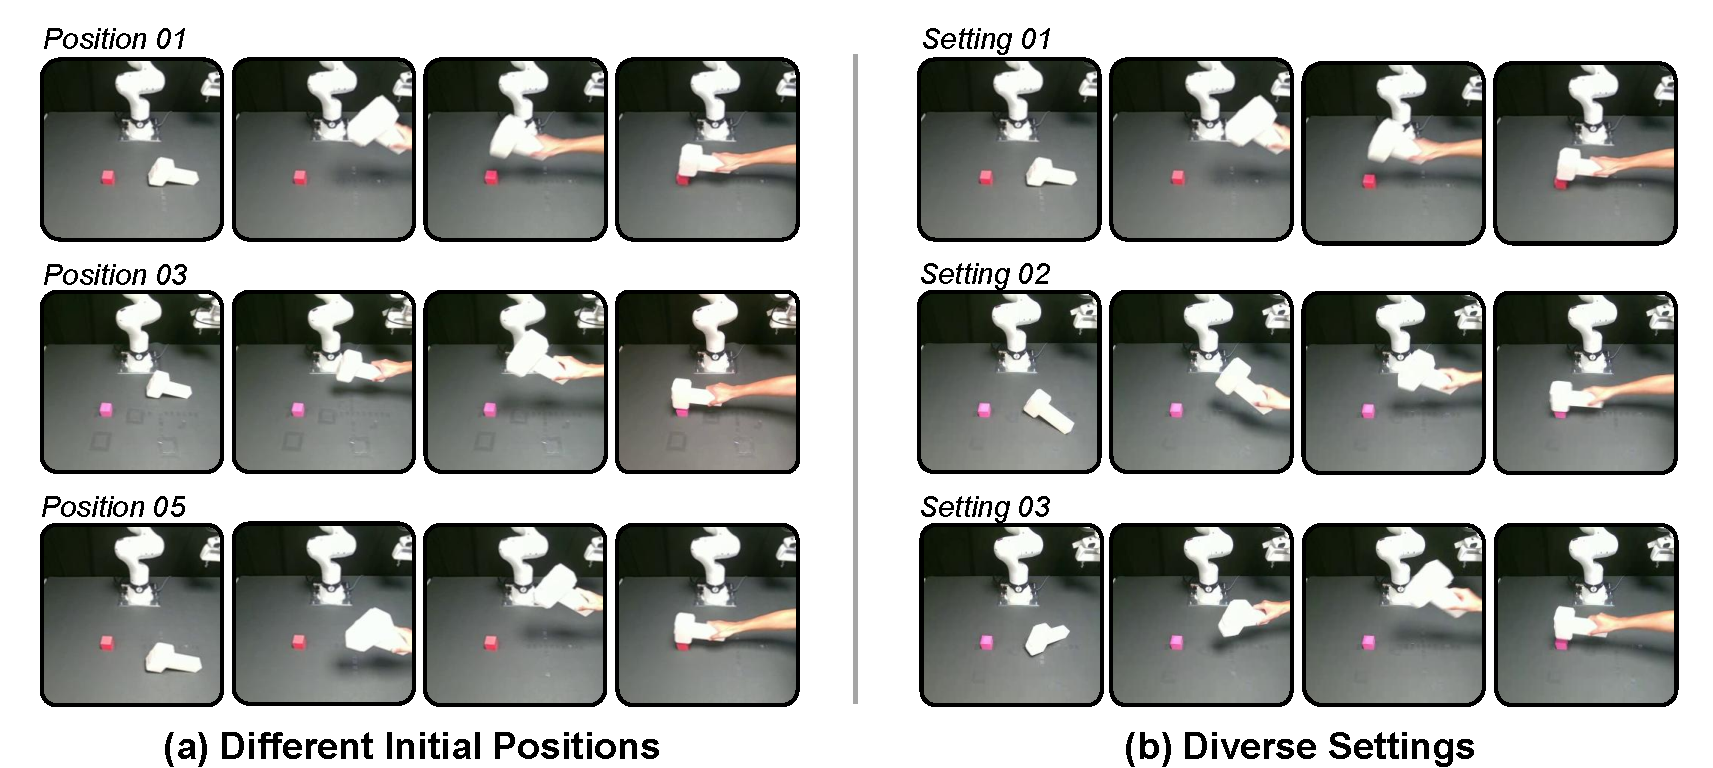
\includegraphics[width=1.0\linewidth]{figures/human-video-prompt.pdf}
    \caption{\textbf{Human Video Prompt Samples.}
    (a) Samples from different initial positions. (b) Samples from different settings.}

    \label{fig:human-video-prompts}
\end{figure}

\textbf{Affordance Images.}~~ 
We manually annotate the grasp point and hitting region for each tool, producing 10 affordance images in total. When evaluating functional intermediate representations in Sec.~\ref{sec:Functional Intermediate Representations Selection}, we use the affordance image of the corresponding tool as an additional condition for the grounded execution policy $\pi_{\mathrm{sys1}}$. Since this representation is time-invariant, the same image feature is shared across all time steps of a trajectory.





\textbf{Human Video Prompts.}~~
As shown in Fig.~\ref{fig:human-video-prompts}, we collect human video prompts for all 7 tools. Following the simulation benchmark, each tool has 3 settings. For each setting, we define 5 initial positions and collect 5 videos per position, resulting in 525 human tool-use videos in total. When evaluating functional intermediate representations, we use the video prompt corresponding to the same tool, setting, and sample from Position 01 as an additional condition for the grounded execution policy. These videos provide visual demonstrations of how humans accomplish the same hitting function with different tools. We further validate that human video data can serve as effective action-free pretraining data for functional reasoning in Sec.~\ref{sec:scalability-human-video}.


\textbf{Functional Videos and Object Masks.}~~
For each simulation demonstration, we use the corresponding ground-truth functional execution video as a temporally varying condition.
To construct object masks, we remove the background from each frame while retaining the tool and target object, thereby preserving object-centric geometry and motion while suppressing background appearance.
Both representations are temporally aligned with the robot trajectory and used as sequential conditions for $\pi_{\mathrm{sys1}}$.
With 10 tools, 3 settings, and 30 randomized initial configurations per setting, we obtain 900 functional-video sequences and 900 object-mask sequences in total.

\textbf{Keypoint Trajectories.}~~
We adopt 2D keypoint trajectories as the final functional intermediate representation and extract them for both simulation and real-world data. In simulation, the hitting and target points are directly obtained from the simulator. Given the initial hitting point on the tool, we use SAM2~\citep{ravi2025sam} to segment the corresponding tool mask and sample $N=5$ additional tool keypoints with Farthest Point Sampling (FPS), ensuring spatial coverage of the tool geometry. We then track these sampled tool keypoints with CoTracker~\citep{karaev2024cotracker} to obtain their 2D trajectories. Our simulation benchmark contains 10 tools with 3 settings each. For each setting, we randomly initialize 30 hitting and target positions, resulting in 900 simulation samples.
For real-world data, we manually annotate the target and hitting points for each sample and obtain five additional tool keypoints using the same SAM2- and FPS-based procedure. Unlike simulation, where the hitting and target trajectories are available from the simulator, all 7 real-world keypoints are tracked by CoTracker. The real-world benchmark contains 7 tools, each with 2 hitting patterns
and 1 initial position. We collect 20 samples for each initial position, resulting in 280 real-world samples. 
% These trajectories are used as action-free supervision, while robot action labels from the evaluation tools are not used to train the execution policy.



\subsection{MPPI-based Demonstration Generation}
\label{app:mppi_annotation}

% In the simulation benchmark, the action-labeled demonstrations are automatically generated rather than collected through teleoperation. We use a Model Predictive Path Integral (MPPI) planner with a four-stage rollout procedure, whose main reward terms are summarized in Tab.~\ref{tab:mppi_rewards}. The stages sequentially encourage the robot to lift the tool, move it toward the target, align the tool-specific hitting point with the target, and execute the final downward strike.
In the simulation benchmark, the action-labeled demonstrations are automatically generated rather than collected through teleoperation.
We use a Model Predictive Path Integral (MPPI) planner with function-specific objectives.
Taking the hitting function as an example, we adopt a four-stage rollout procedure, whose detailed reward terms are summarized in Tab.~\ref{tab:mppi_rewards}.
The stages sequentially encourage the robot to lift the tool, move it toward the target, align the tool-specific hitting point with the target, and execute the final downward strike.

Besides the translational commands optimized by MPPI, we specify a target rotational pose at the end of each stage and generate the corresponding rotational commands through servo control. This helps the tool maintain an appropriate orientation during lifting, alignment, and hitting. Together, the stage-specific MPPI rewards and rotational servo control enable reliable automatic demonstration generation in simulation.


\begin{table}[p]
\centering
\caption{\textbf{Main Reward Terms for MPPI-based Demonstration Generation.}
Here, $d_x$, $d_y$, and $d_{xy}$ denote the distances between the hitting point and the target along the $x$ axis, the $y$ axis, and the $xy$ plane, respectively, while $\Delta d_x$, $\Delta d_y$, and $\Delta d_{xy}$ denote their step-wise reductions.
For the vertical direction, $z_{\mathrm{lift}}$ denotes the tool lifting height from its initial height, $z_1$ denotes the target lifting threshold in Stage~1, $\Delta z_{\mathrm{lift}}$ denotes the step-wise lifting progress, and $e_z$ denotes the error between the current tool height and the target hovering height.
$\Delta z_{\mathrm{head}}$ denotes the vertical displacement of the hitting point between consecutive steps, so $-\Delta z_{\mathrm{head}}$ measures downward motion.
The terms $r_\ast$ reward the current state for satisfying the stage-specific objective, while $r_{\ast\_\mathrm{prog}}$ rewards step-wise progress toward that objective.}

\label{tab:mppi_rewards}
\resizebox{\linewidth}{!}{
\begin{tabular}{lp{0.30\linewidth}p{0.50\linewidth}}
\toprule
Stage & Objective & Main Reward Terms \\
\midrule
Stage 1 
& Lift the tool and align it with the target along the $x$ and $y$ axes.
& 
$
\begin{aligned}
r_{\mathrm{lift}} &= 18.0\min(z_{\mathrm{lift}}, z_1), \\
r_{\mathrm{lift\_prog}} &= 100.0\min(\Delta z_{\mathrm{lift}}, 0.02), \\
r_x &= 22.0\exp(-18.0 d_x), \\
r_{x\_\mathrm{prog}} &= 120.0\min(\Delta d_x, 0.02), \\
r_y &= 8.0\exp(-8.0 d_y), \\
r_{y\_\mathrm{prog}} &= 35.0\min(\Delta d_y, 0.02).
\end{aligned}
$
\\
\midrule
Stage 2 
& Move the tool toward the target while maintaining a suitable hovering height. 
& 
$
\begin{aligned}
r_{xy} &= 14.0\exp(-10.0 d_{xy}), \\
r_x &= 12.0\exp(-18.0 d_x), \\
r_y &= 8.0\exp(-10.0 d_y), \\
r_z &= 7.0\exp(-18.0 e_z), \\
r_{xy\_\mathrm{prog}} &= 95.0\min(\Delta d_{xy}, 0.02), \\
r_{x\_\mathrm{prog}} &= 80.0\min(\Delta d_x, 0.02), \\
r_{y\_\mathrm{prog}} &= 40.0\min(\Delta d_y, 0.02).
\end{aligned}
$
\\
\midrule
Stage 3 
& Finely align the tool-specific hitting point above the target. 
& 
$
\begin{aligned}
r_{xy} &= 14.0\exp(-14.0 d_{xy}), \\
r_x &= 14.0\exp(-24.0 d_x), \\
r_y &= 10.0\exp(-18.0 d_y), \\
r_{xy\_\mathrm{prog}} &= 145.0\min(\Delta d_{xy}, 0.018), \\
r_{x\_\mathrm{prog}} &= 135.0\min(\Delta d_x, 0.018), \\
r_{y\_\mathrm{prog}} &= 110.0\min(\Delta d_y, 0.018), \\
r_z &= 7.0\exp(-18.0 e_z).
\end{aligned}
$
\\
\midrule
Stage 4 
& Keep the hitting point close to the target and execute the downward strike. 
& 
$
\begin{aligned}
r_{xy} &= 12.0\exp(-16.0 d_{xy}), \\
r_x &= 14.0\exp(-28.0 d_x), \\
r_y &= 10.0\exp(-18.0 d_y), \\
r_{xy\_\mathrm{prog}} &= 120.0\min(\Delta d_{xy}, 0.015), \\
r_{x\_\mathrm{prog}} &= 100.0\min(\Delta d_x, 0.015), \\
r_{y\_\mathrm{prog}} &= 80.0\min(\Delta d_y, 0.015), \\
r_{\mathrm{hit}} &= 150.0\min(-\Delta z_{\mathrm{head}}, 0.05),
\end{aligned}
$
\\
\midrule
Contact / Success 
& Encourage valid downward contact with the target.
& 
$
\begin{aligned}
r_{\mathrm{contact}} &= 150.0 \ \text{if valid downward contact}.
\end{aligned}
$
\\
\bottomrule
\end{tabular}
}
\end{table}
\FloatBarrier

\subsection{Training and Implementation Details}
\label{app:implementation_details}

All models are trained on NVIDIA RTX 6000 Pro GPUs. For all methods, we use an action chunk size of 8, a history horizon of 8, and a batch size of 64. We build the simulation benchmark on Robomimic and conduct real-world experiments on a Franka robot platform.

For baseline methods, we train each policy for 120,000 steps using the corresponding action-labeled data. For \algoname{}, we follow the two-stage training procedure described in Sec.~\ref{sec:FORGE}. 
%We first pretrain the keypoint motion predictor $\pi_{\mathrm{sys2}}$ on action-free data from all tools for 240,000 steps.
We first pretrain the keypoint motion predictor $\pi_{\mathrm{sys2}}$ on independently collected action-free data for 240,000 steps.
We then freeze the pretrained predictor and fine-tune the grounded execution policy $\pi_{\mathrm{sys1}}$ on the same action-labeled data used by the baselines for 120,000 steps.


\section{Additional Experimental Results}
\label{app:additional_experimental_results}

This section provides additional qualitative comparisons across hitting, sweeping, and hooking in both the real world and simulation. These results complement the quantitative evaluations in the main paper by illustrating representative failure modes of the baselines and how \algoname{} addresses them through function-aware keypoint motion planning.

\begin{figure}[!htbp]
    \centering
    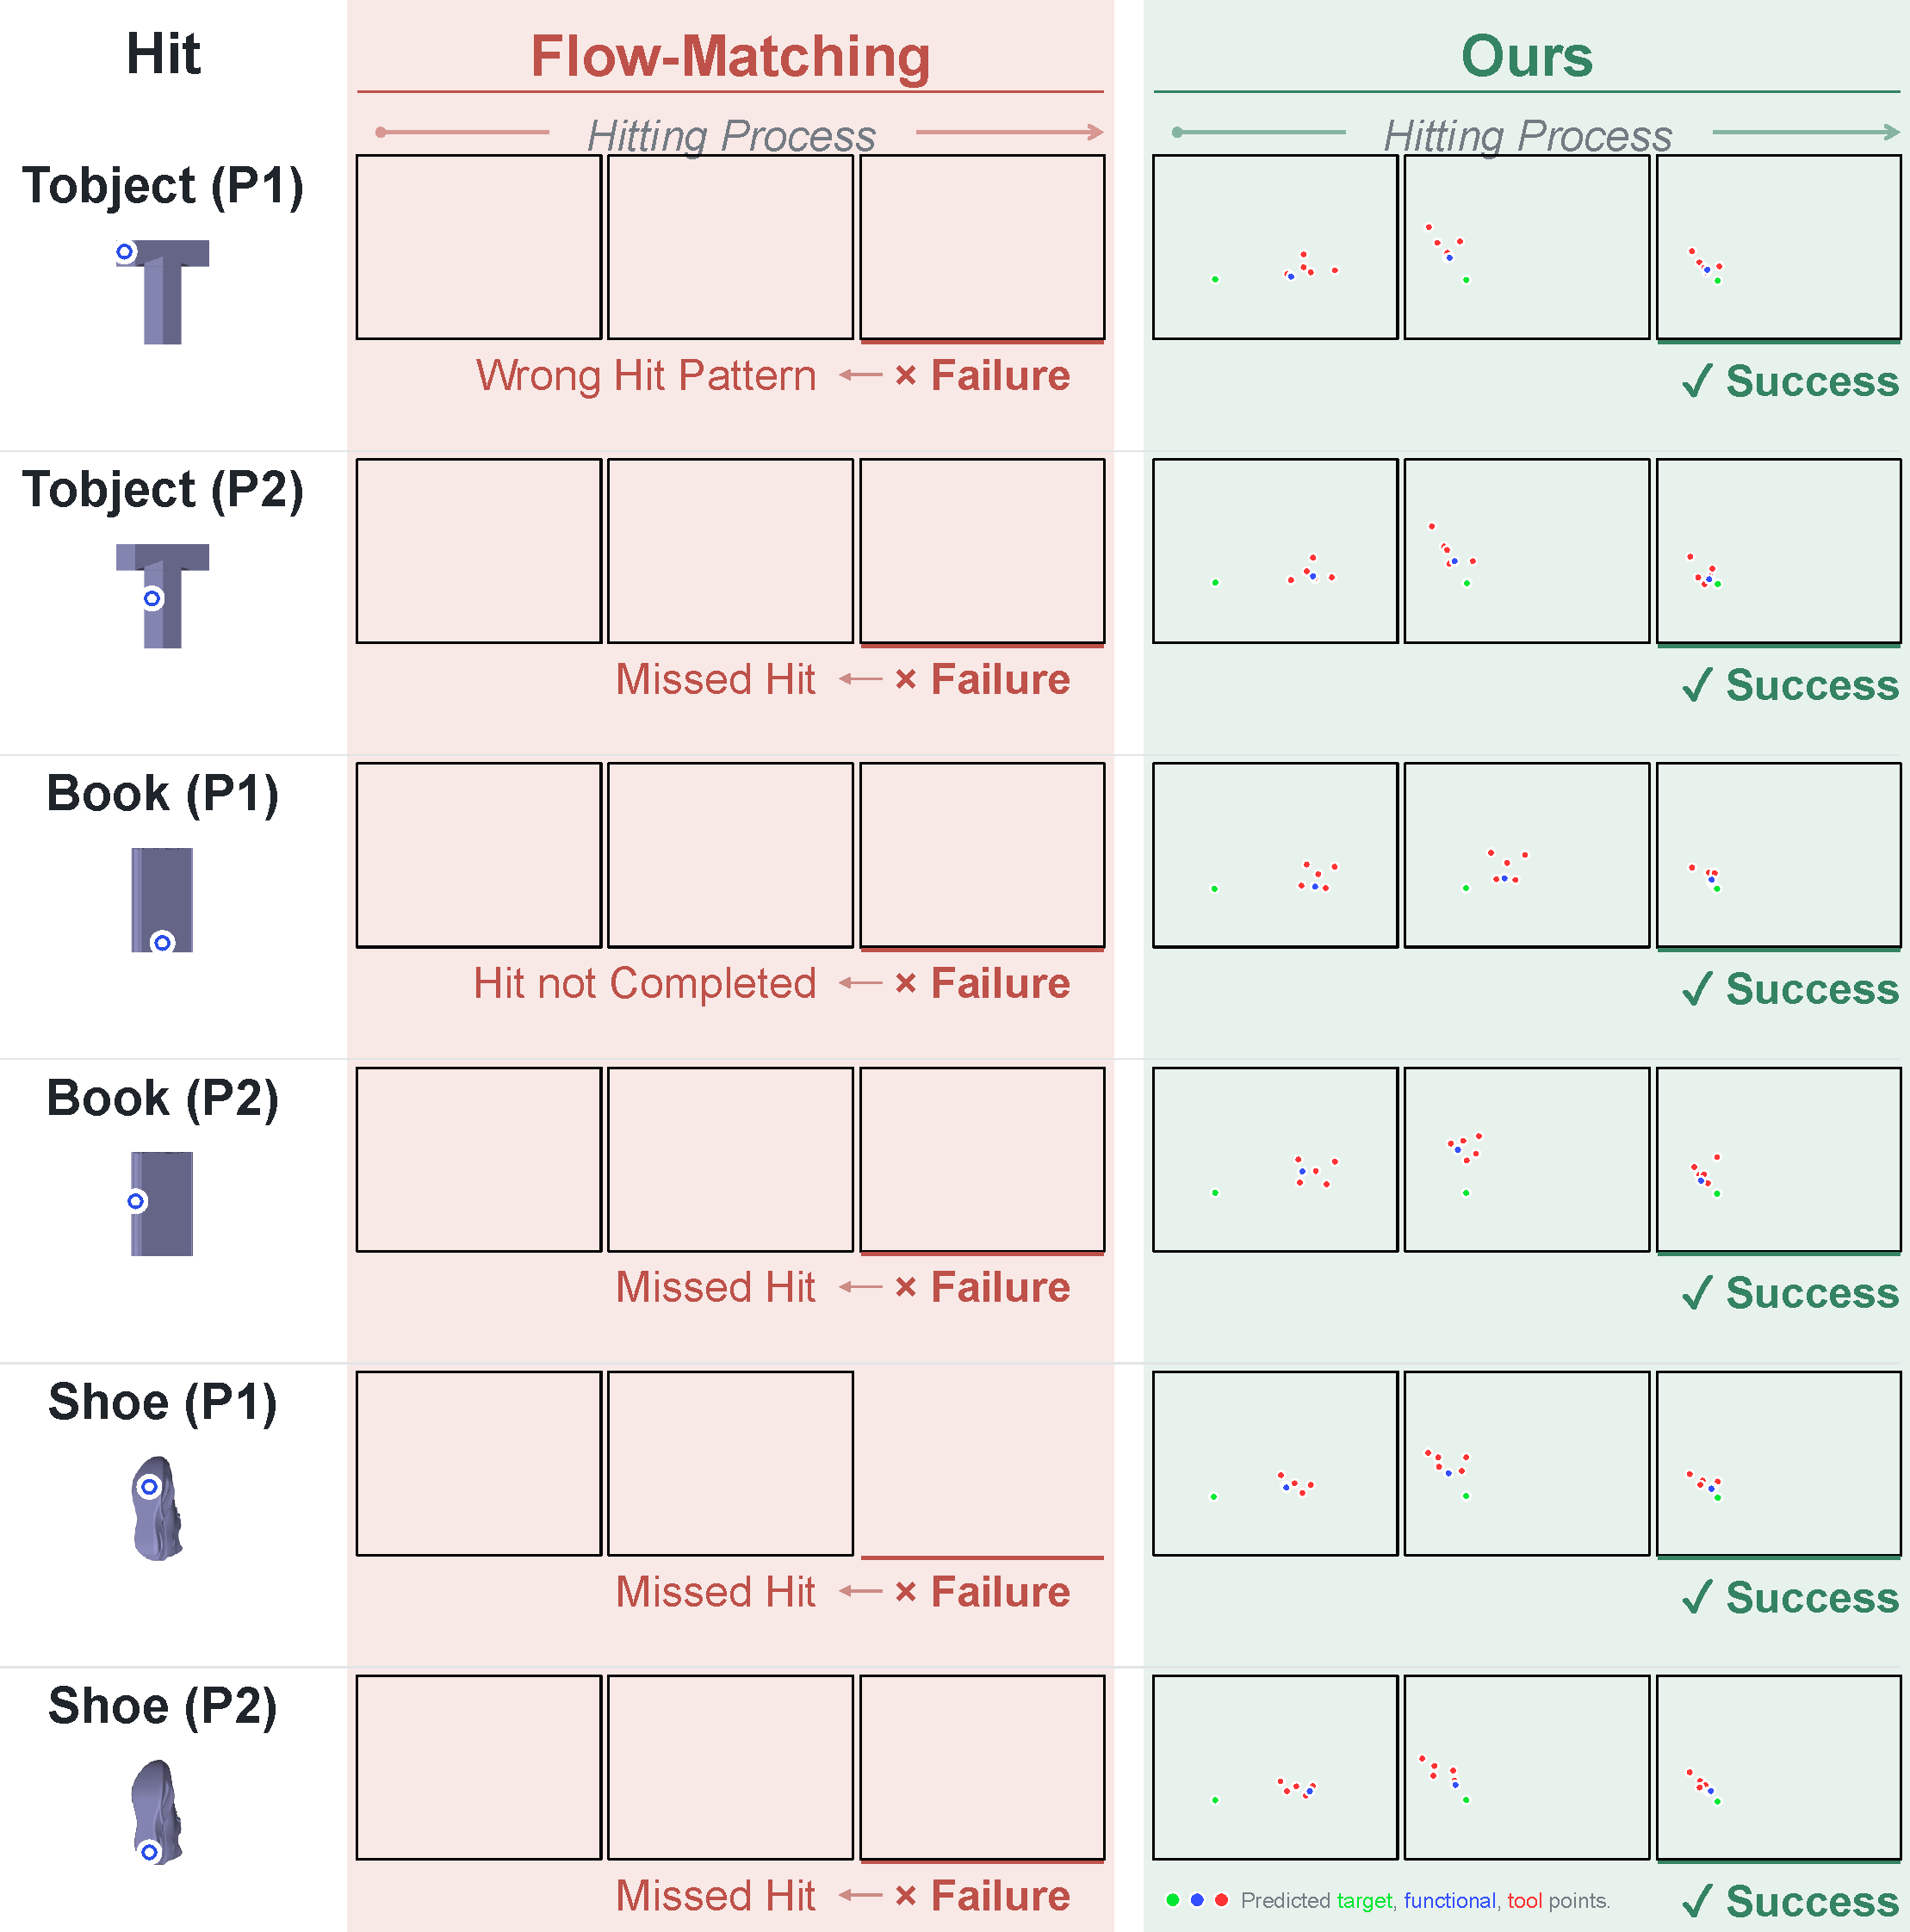
\includegraphics[width=0.82\linewidth]{figures/app-hitting-real.pdf}
    \caption{\textbf{Real-World Qualitative Results for Hitting.} Failures of the FM baseline and successful demos of \algoname{} on unseen tools across hitting patterns. The blue point indicates the reference hitting point for each pattern.}
    \label{fig:app-real-hitting}
\end{figure}

\begin{figure}[!htbp]
    \centering
    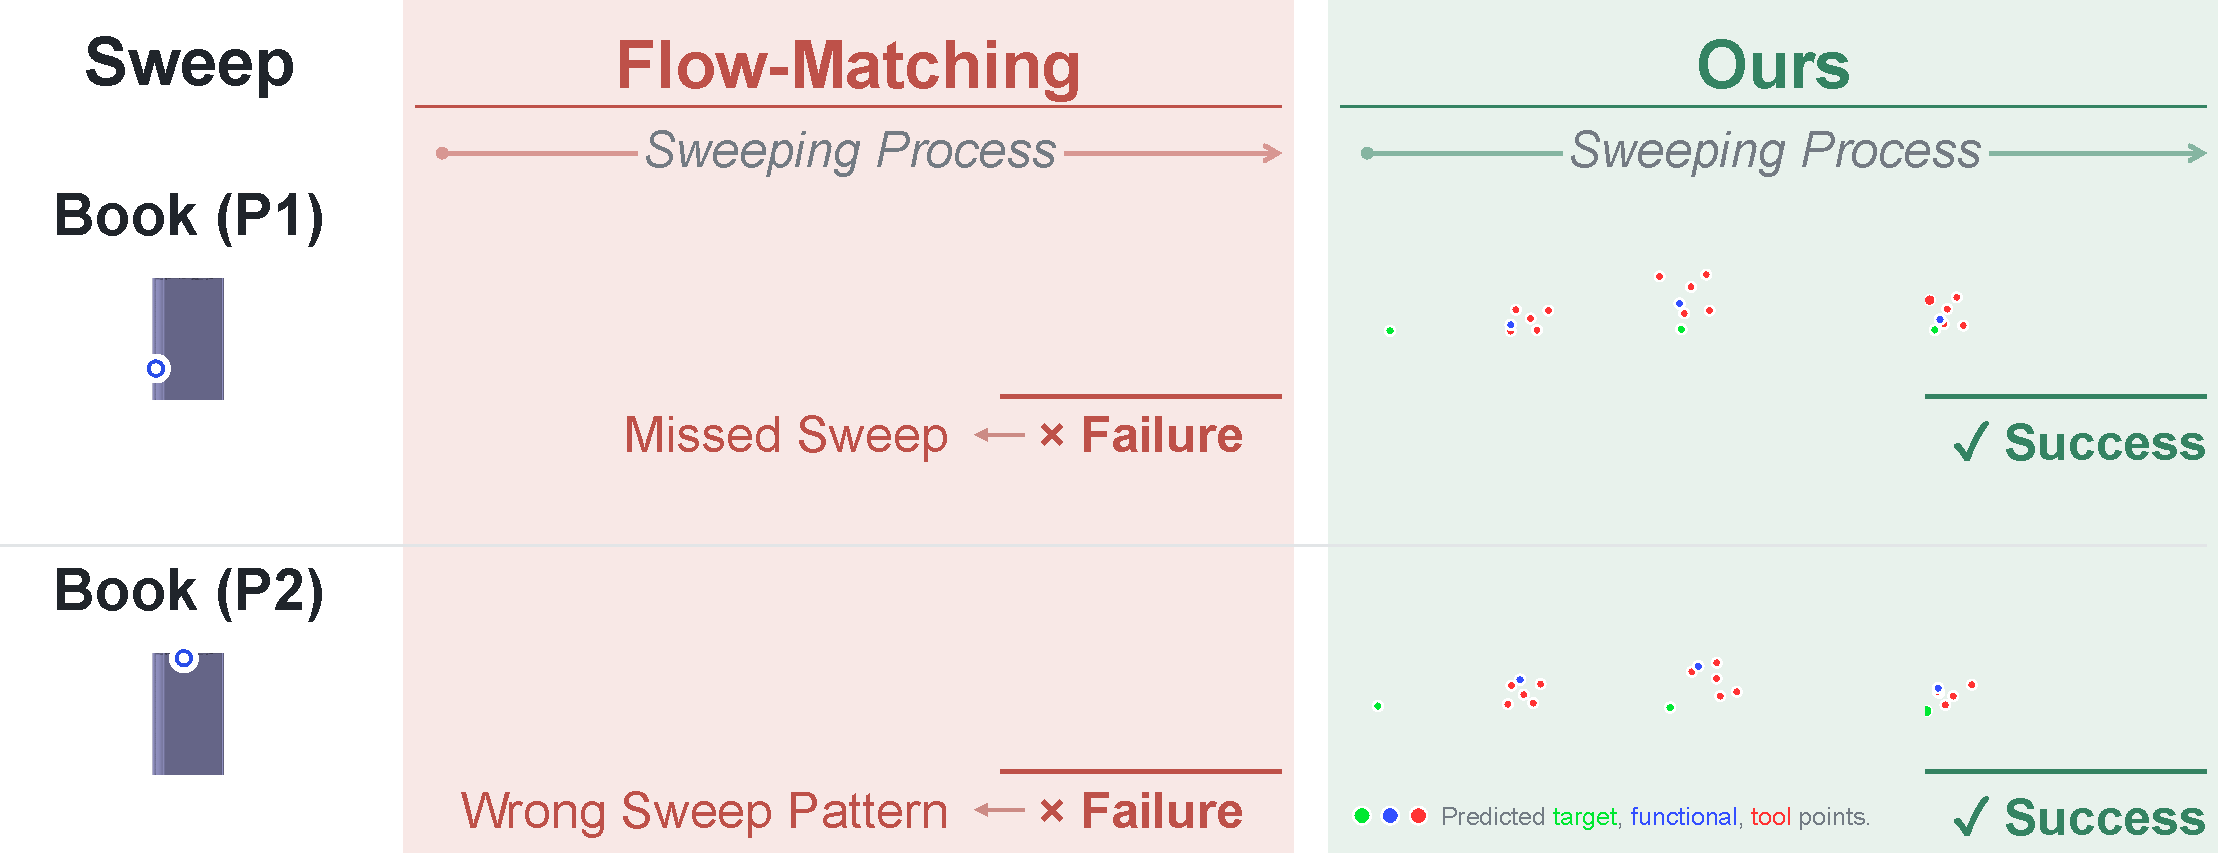
\includegraphics[width=0.82\linewidth]{figures/app-sweeping-real.pdf}
    \caption{\textbf{Real-World Qualitative Results for Sweeping.} Failures of the FM baseline and successful demos of \algoname{} on unseen tools across sweeping patterns. The blue point indicates the reference sweeping point for each pattern.}
    \label{fig:app-real-sweeping}
\end{figure}

\begin{figure}[!htbp]
    \centering
    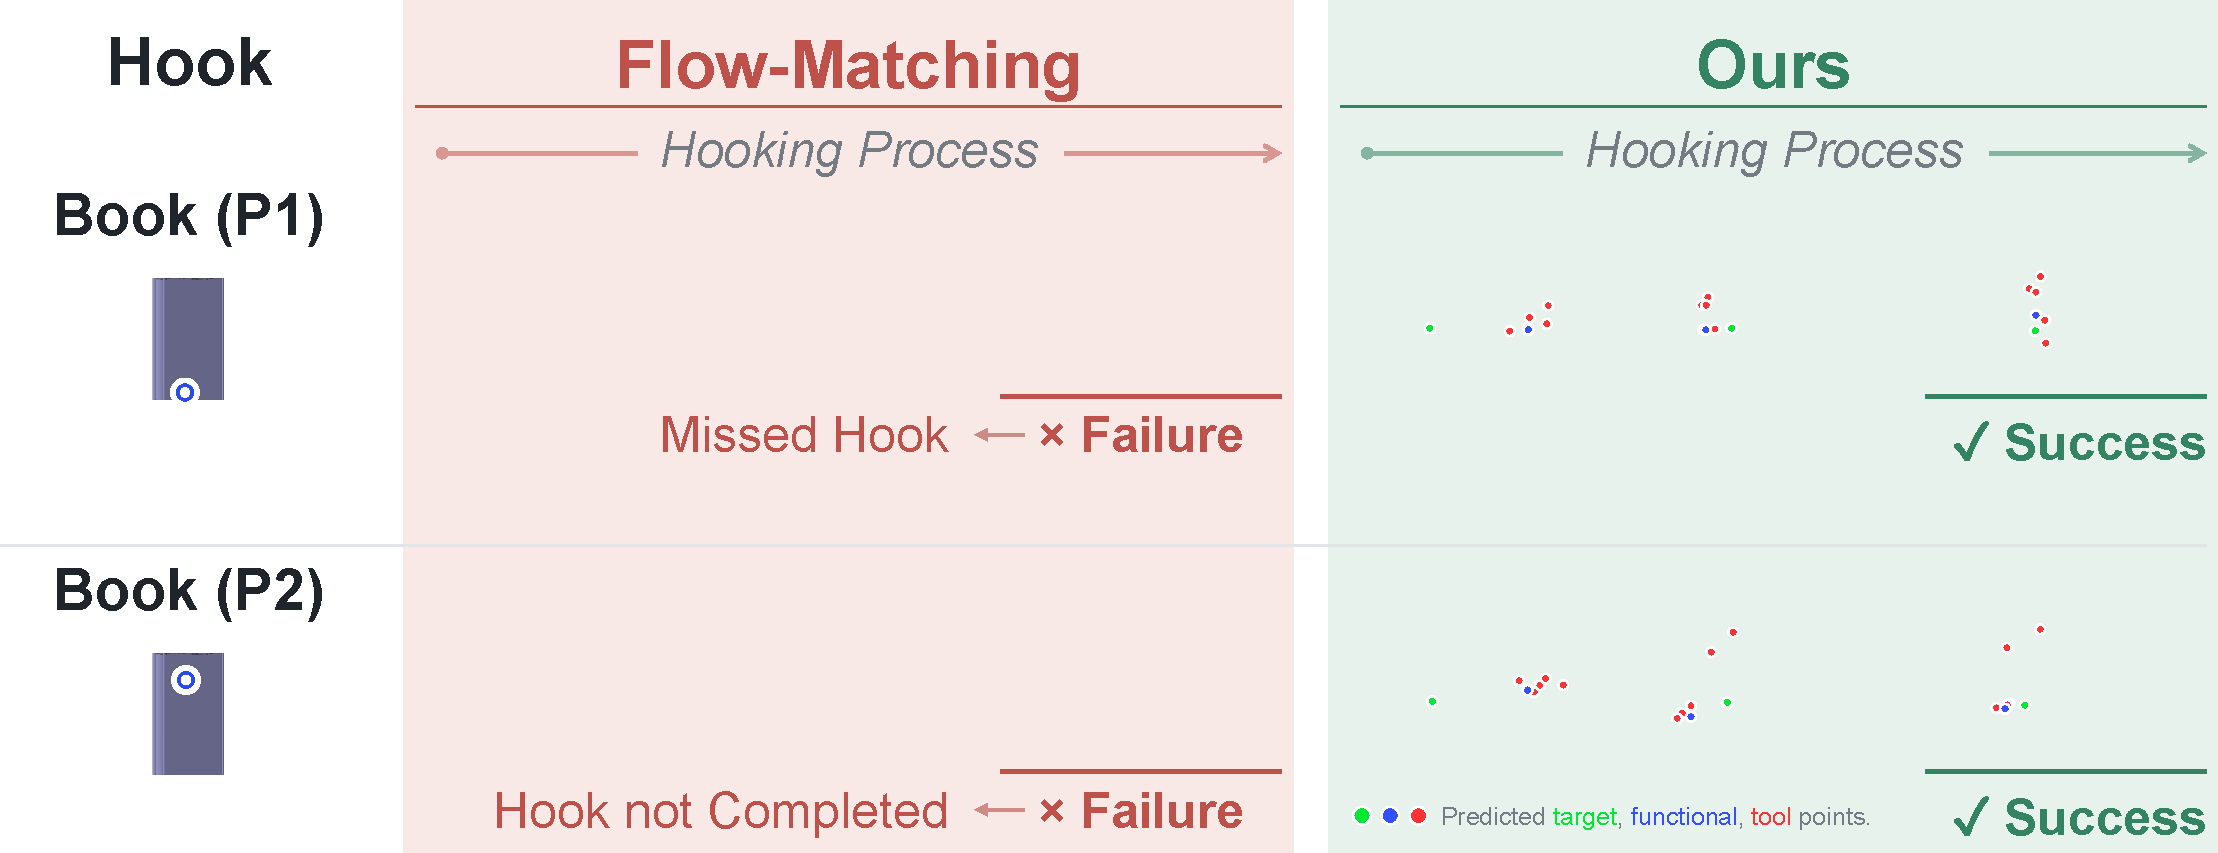
\includegraphics[width=0.82\linewidth]{figures/app-hooking-real.pdf}
    \caption{\textbf{Real-World Qualitative Results for Hooking.} Failures of the FM baseline and successful demos of \algoname{} on unseen tools across hooking patterns. The blue point indicates the reference hooking point for each pattern.}
     \label{fig:app-real-hooking}
\end{figure}


\FloatBarrier
\subsection{More Qualitative Results in the Real World}
\label{app:more_qualitative_results_real}

Figs.~\ref{fig:app-real-hitting}--\ref{fig:app-real-hooking} provide additional real-world comparisons between the FM baseline and \algoname{} across hitting, sweeping, and hooking on unseen tools and different functional patterns.
Across the three functions, FM exhibits representative failure modes including missed or incomplete interactions and incorrect functional motion patterns, showing that an end-to-end policy struggles to adapt both the functional region and the required motion to novel tool geometries.
By contrast, \algoname{} uses predicted keypoint-based functional plans to guide functional-region alignment and motion execution, leading to successful interactions across the shown hitting, sweeping, and hooking cases.
These results further demonstrate the benefit of an explicit function-aware intermediate representation for functional generalization.



\begin{figure}[!htbp]
    \centering
    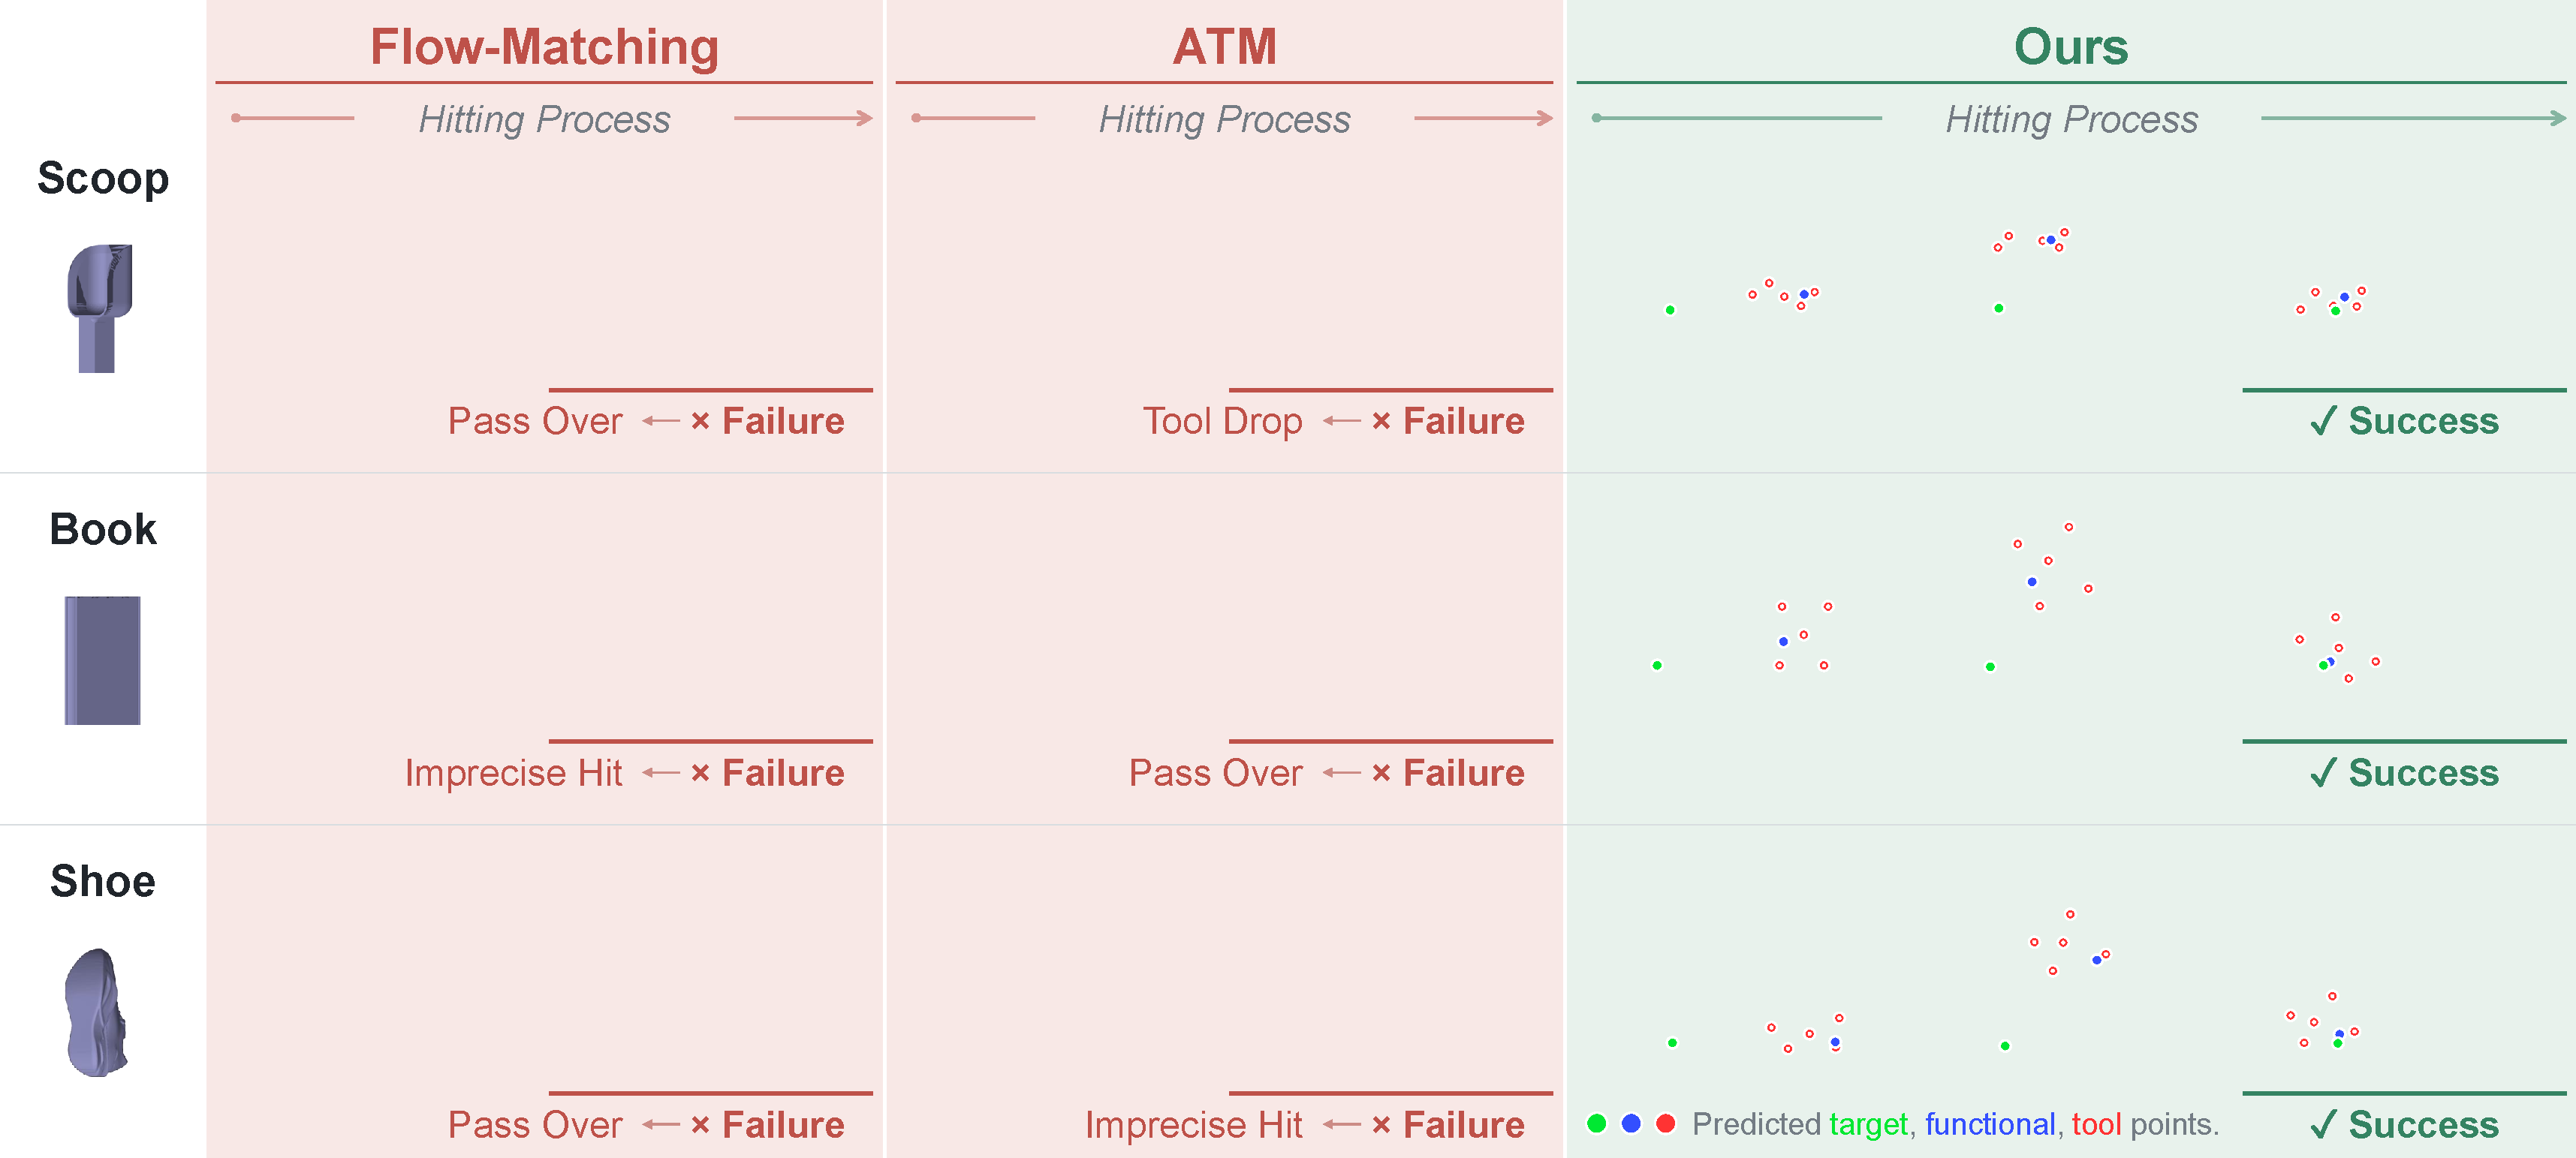
\includegraphics[width=0.82\linewidth]{figures/app-hitting-sim.pdf}
    \caption{\textbf{Simulation Qualitative Results for Hitting.} Failures of FM and ATM and successful rollouts of \algoname{} on unseen tools.}
    \label{fig:app-hitting-sim}
\end{figure}

\begin{figure}[!htbp]
    \centering
    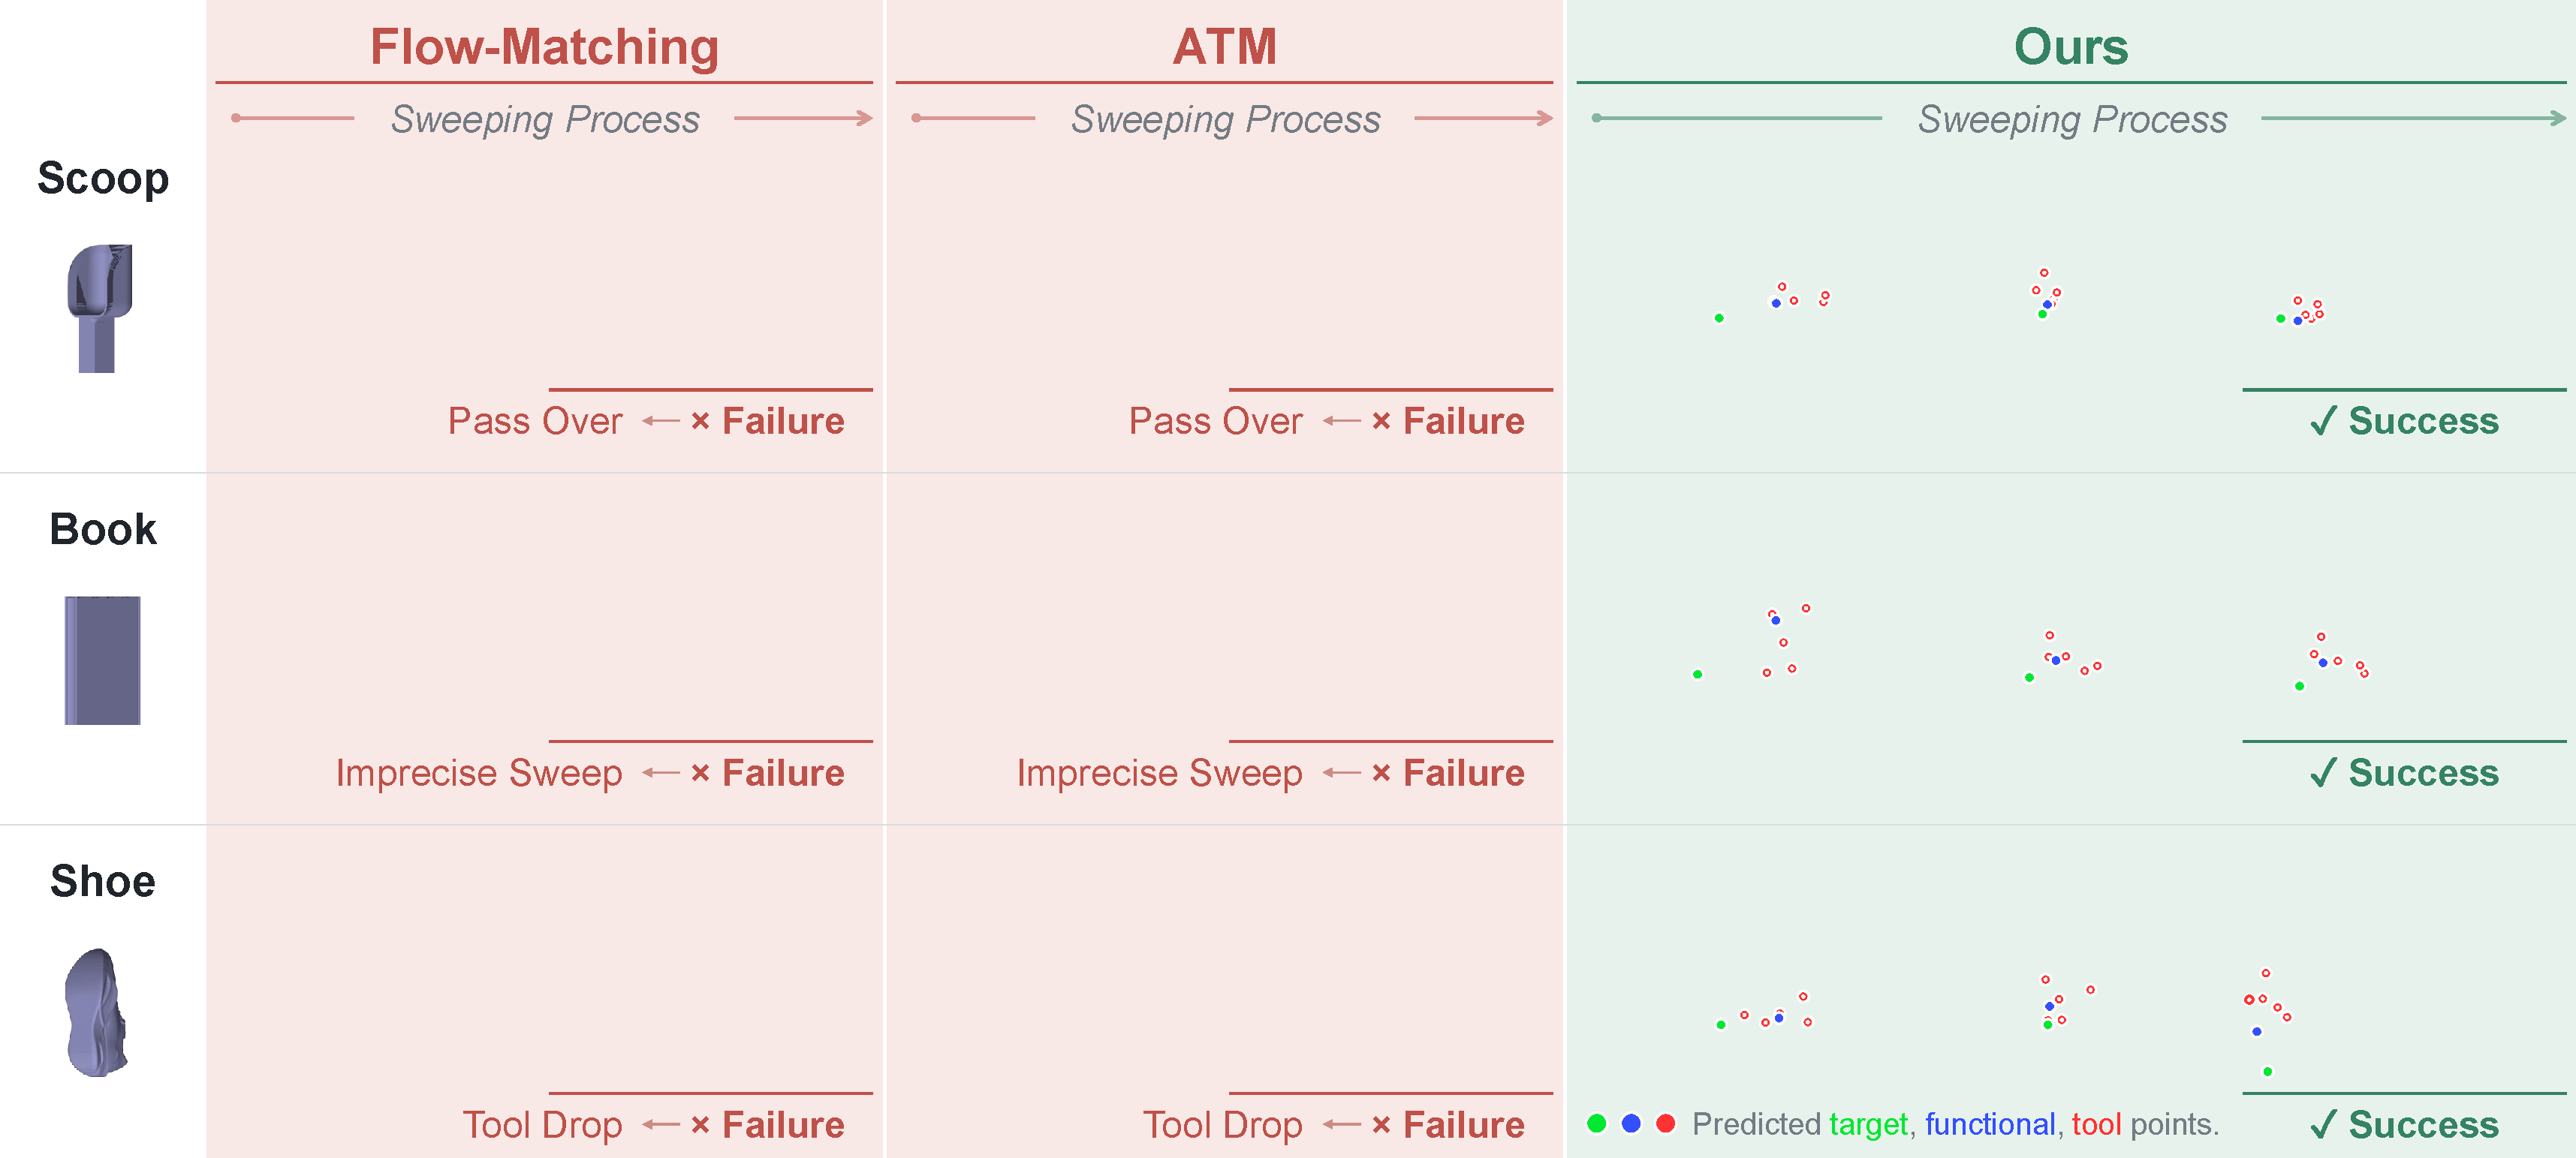
\includegraphics[width=0.82\linewidth]{figures/app-sweeping-sim.pdf}
    \caption{\textbf{Simulation Qualitative Results for Sweeping.} Failures of FM and ATM and successful rollouts of \algoname{} on unseen tools.}
    \label{fig:app-sweeping-sim}
\end{figure}

\begin{figure}[!htbp]
    \centering
    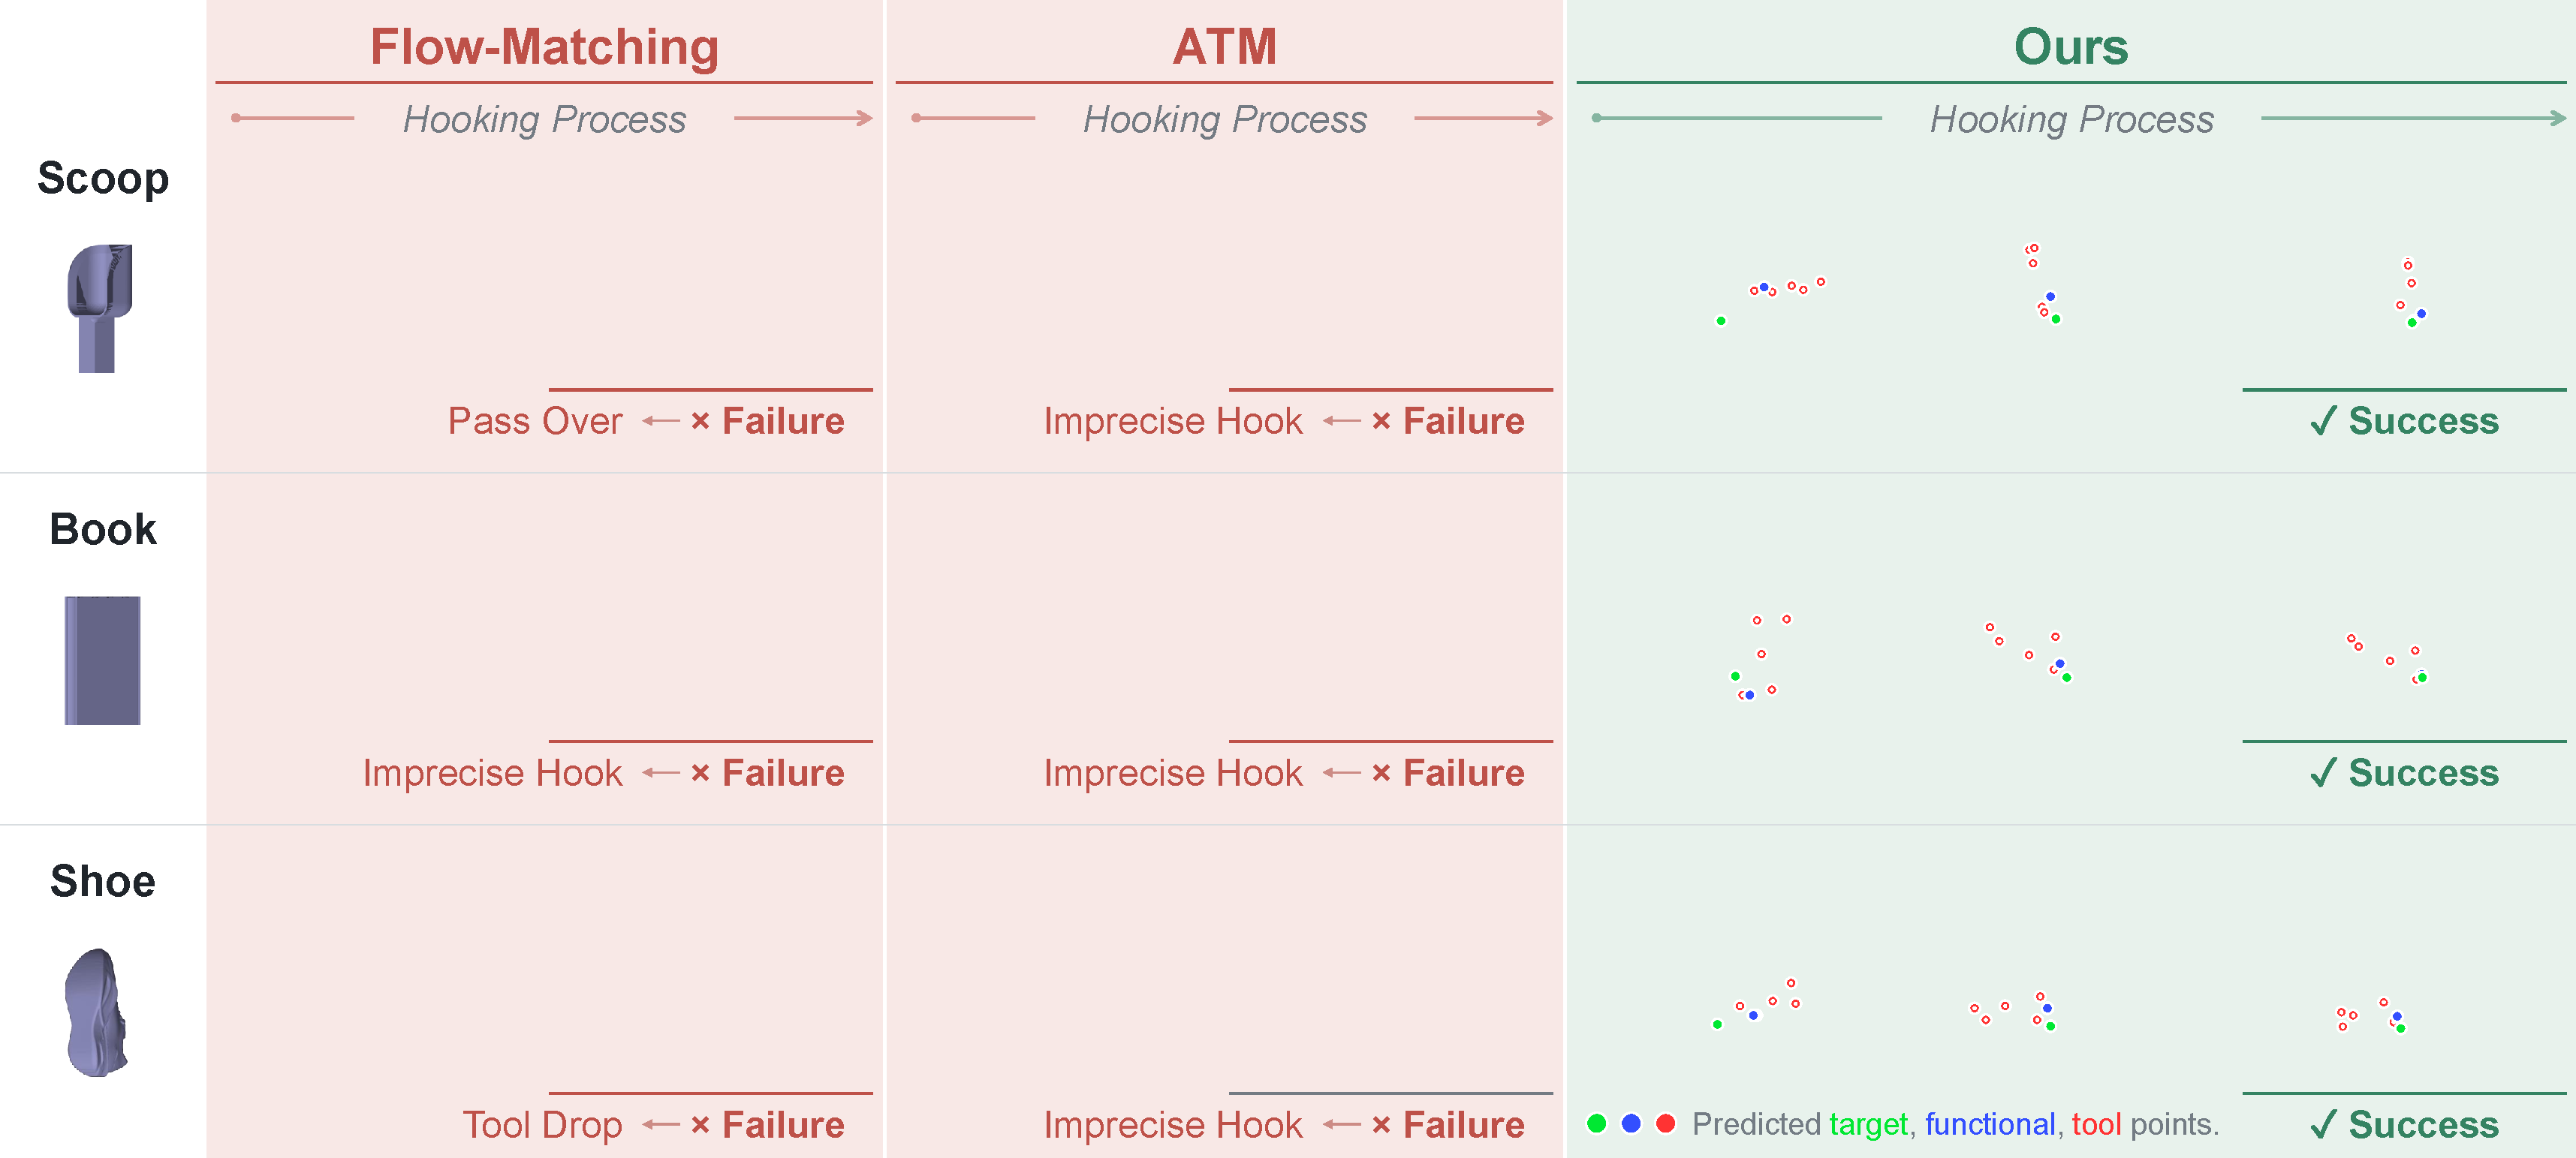
\includegraphics[width=0.82\linewidth]{figures/app-hooking-sim.pdf}
    \caption{\textbf{Simulation Qualitative Results for Hooking.} Failures of FM and ATM and successful rollouts of \algoname{} on unseen tools.}
    \label{fig:app-hooking-sim}
\end{figure}


\FloatBarrier
\subsection{More Qualitative Results in Simulation}
\label{app:more_qualitative_results_sim}

Figs.~\ref{fig:app-hitting-sim}--\ref{fig:app-hooking-sim} provide additional simulation comparisons among FM, ATM, and \algoname{} across hitting, sweeping, and hooking on unseen tools.
FM exhibits representative failures such as passing over the target, imprecise interactions, and tool dropping.
Although ATM also conditions on keypoint trajectories, its generic trajectories do not explicitly encode function-specific motion intent and can therefore exhibit similar failures.
In contrast, \algoname{} predicts function-aware keypoint trajectories that explicitly guide how the functional region should move toward and interact with the target, enabling more reliable execution across the three functions.


Please refer to our supplementary videos for complete rollouts of both simulation and real-world experiments.

\end{document}
